% Options for packages loaded elsewhere
% Options for packages loaded elsewhere
\PassOptionsToPackage{unicode}{hyperref}
\PassOptionsToPackage{hyphens}{url}
\PassOptionsToPackage{dvipsnames,svgnames,x11names}{xcolor}
%
\documentclass[
  brazilian,
  letterpaper,
  DIV=11,
  numbers=noendperiod]{scrartcl}
\usepackage{xcolor}
\usepackage{amsmath,amssymb}
\setcounter{secnumdepth}{-\maxdimen} % remove section numbering
\usepackage{iftex}
\ifPDFTeX
  \usepackage[T1]{fontenc}
  \usepackage[utf8]{inputenc}
  \usepackage{textcomp} % provide euro and other symbols
\else % if luatex or xetex
  \usepackage{unicode-math} % this also loads fontspec
  \defaultfontfeatures{Scale=MatchLowercase}
  \defaultfontfeatures[\rmfamily]{Ligatures=TeX,Scale=1}
\fi
\usepackage{lmodern}
\ifPDFTeX\else
  % xetex/luatex font selection
\fi
% Use upquote if available, for straight quotes in verbatim environments
\IfFileExists{upquote.sty}{\usepackage{upquote}}{}
\IfFileExists{microtype.sty}{% use microtype if available
  \usepackage[]{microtype}
  \UseMicrotypeSet[protrusion]{basicmath} % disable protrusion for tt fonts
}{}
\makeatletter
\@ifundefined{KOMAClassName}{% if non-KOMA class
  \IfFileExists{parskip.sty}{%
    \usepackage{parskip}
  }{% else
    \setlength{\parindent}{0pt}
    \setlength{\parskip}{6pt plus 2pt minus 1pt}}
}{% if KOMA class
  \KOMAoptions{parskip=half}}
\makeatother
% Make \paragraph and \subparagraph free-standing
\makeatletter
\ifx\paragraph\undefined\else
  \let\oldparagraph\paragraph
  \renewcommand{\paragraph}{
    \@ifstar
      \xxxParagraphStar
      \xxxParagraphNoStar
  }
  \newcommand{\xxxParagraphStar}[1]{\oldparagraph*{#1}\mbox{}}
  \newcommand{\xxxParagraphNoStar}[1]{\oldparagraph{#1}\mbox{}}
\fi
\ifx\subparagraph\undefined\else
  \let\oldsubparagraph\subparagraph
  \renewcommand{\subparagraph}{
    \@ifstar
      \xxxSubParagraphStar
      \xxxSubParagraphNoStar
  }
  \newcommand{\xxxSubParagraphStar}[1]{\oldsubparagraph*{#1}\mbox{}}
  \newcommand{\xxxSubParagraphNoStar}[1]{\oldsubparagraph{#1}\mbox{}}
\fi
\makeatother

\usepackage{color}
\usepackage{fancyvrb}
\newcommand{\VerbBar}{|}
\newcommand{\VERB}{\Verb[commandchars=\\\{\}]}
\DefineVerbatimEnvironment{Highlighting}{Verbatim}{commandchars=\\\{\}}
% Add ',fontsize=\small' for more characters per line
\usepackage{framed}
\definecolor{shadecolor}{RGB}{241,243,245}
\newenvironment{Shaded}{\begin{snugshade}}{\end{snugshade}}
\newcommand{\AlertTok}[1]{\textcolor[rgb]{0.68,0.00,0.00}{#1}}
\newcommand{\AnnotationTok}[1]{\textcolor[rgb]{0.37,0.37,0.37}{#1}}
\newcommand{\AttributeTok}[1]{\textcolor[rgb]{0.40,0.45,0.13}{#1}}
\newcommand{\BaseNTok}[1]{\textcolor[rgb]{0.68,0.00,0.00}{#1}}
\newcommand{\BuiltInTok}[1]{\textcolor[rgb]{0.00,0.23,0.31}{#1}}
\newcommand{\CharTok}[1]{\textcolor[rgb]{0.13,0.47,0.30}{#1}}
\newcommand{\CommentTok}[1]{\textcolor[rgb]{0.37,0.37,0.37}{#1}}
\newcommand{\CommentVarTok}[1]{\textcolor[rgb]{0.37,0.37,0.37}{\textit{#1}}}
\newcommand{\ConstantTok}[1]{\textcolor[rgb]{0.56,0.35,0.01}{#1}}
\newcommand{\ControlFlowTok}[1]{\textcolor[rgb]{0.00,0.23,0.31}{\textbf{#1}}}
\newcommand{\DataTypeTok}[1]{\textcolor[rgb]{0.68,0.00,0.00}{#1}}
\newcommand{\DecValTok}[1]{\textcolor[rgb]{0.68,0.00,0.00}{#1}}
\newcommand{\DocumentationTok}[1]{\textcolor[rgb]{0.37,0.37,0.37}{\textit{#1}}}
\newcommand{\ErrorTok}[1]{\textcolor[rgb]{0.68,0.00,0.00}{#1}}
\newcommand{\ExtensionTok}[1]{\textcolor[rgb]{0.00,0.23,0.31}{#1}}
\newcommand{\FloatTok}[1]{\textcolor[rgb]{0.68,0.00,0.00}{#1}}
\newcommand{\FunctionTok}[1]{\textcolor[rgb]{0.28,0.35,0.67}{#1}}
\newcommand{\ImportTok}[1]{\textcolor[rgb]{0.00,0.46,0.62}{#1}}
\newcommand{\InformationTok}[1]{\textcolor[rgb]{0.37,0.37,0.37}{#1}}
\newcommand{\KeywordTok}[1]{\textcolor[rgb]{0.00,0.23,0.31}{\textbf{#1}}}
\newcommand{\NormalTok}[1]{\textcolor[rgb]{0.00,0.23,0.31}{#1}}
\newcommand{\OperatorTok}[1]{\textcolor[rgb]{0.37,0.37,0.37}{#1}}
\newcommand{\OtherTok}[1]{\textcolor[rgb]{0.00,0.23,0.31}{#1}}
\newcommand{\PreprocessorTok}[1]{\textcolor[rgb]{0.68,0.00,0.00}{#1}}
\newcommand{\RegionMarkerTok}[1]{\textcolor[rgb]{0.00,0.23,0.31}{#1}}
\newcommand{\SpecialCharTok}[1]{\textcolor[rgb]{0.37,0.37,0.37}{#1}}
\newcommand{\SpecialStringTok}[1]{\textcolor[rgb]{0.13,0.47,0.30}{#1}}
\newcommand{\StringTok}[1]{\textcolor[rgb]{0.13,0.47,0.30}{#1}}
\newcommand{\VariableTok}[1]{\textcolor[rgb]{0.07,0.07,0.07}{#1}}
\newcommand{\VerbatimStringTok}[1]{\textcolor[rgb]{0.13,0.47,0.30}{#1}}
\newcommand{\WarningTok}[1]{\textcolor[rgb]{0.37,0.37,0.37}{\textit{#1}}}

\usepackage{longtable,booktabs,array}
\usepackage{calc} % for calculating minipage widths
% Correct order of tables after \paragraph or \subparagraph
\usepackage{etoolbox}
\makeatletter
\patchcmd\longtable{\par}{\if@noskipsec\mbox{}\fi\par}{}{}
\makeatother
% Allow footnotes in longtable head/foot
\IfFileExists{footnotehyper.sty}{\usepackage{footnotehyper}}{\usepackage{footnote}}
\makesavenoteenv{longtable}
\usepackage{graphicx}
\makeatletter
\newsavebox\pandoc@box
\newcommand*\pandocbounded[1]{% scales image to fit in text height/width
  \sbox\pandoc@box{#1}%
  \Gscale@div\@tempa{\textheight}{\dimexpr\ht\pandoc@box+\dp\pandoc@box\relax}%
  \Gscale@div\@tempb{\linewidth}{\wd\pandoc@box}%
  \ifdim\@tempb\p@<\@tempa\p@\let\@tempa\@tempb\fi% select the smaller of both
  \ifdim\@tempa\p@<\p@\scalebox{\@tempa}{\usebox\pandoc@box}%
  \else\usebox{\pandoc@box}%
  \fi%
}
% Set default figure placement to htbp
\def\fps@figure{htbp}
\makeatother


% definitions for citeproc citations
\NewDocumentCommand\citeproctext{}{}
\NewDocumentCommand\citeproc{mm}{%
  \begingroup\def\citeproctext{#2}\cite{#1}\endgroup}
\makeatletter
 % allow citations to break across lines
 \let\@cite@ofmt\@firstofone
 % avoid brackets around text for \cite:
 \def\@biblabel#1{}
 \def\@cite#1#2{{#1\if@tempswa , #2\fi}}
\makeatother
\newlength{\cslhangindent}
\setlength{\cslhangindent}{1.5em}
\newlength{\csllabelwidth}
\setlength{\csllabelwidth}{3em}
\newenvironment{CSLReferences}[2] % #1 hanging-indent, #2 entry-spacing
 {\begin{list}{}{%
  \setlength{\itemindent}{0pt}
  \setlength{\leftmargin}{0pt}
  \setlength{\parsep}{0pt}
  % turn on hanging indent if param 1 is 1
  \ifodd #1
   \setlength{\leftmargin}{\cslhangindent}
   \setlength{\itemindent}{-1\cslhangindent}
  \fi
  % set entry spacing
  \setlength{\itemsep}{#2\baselineskip}}}
 {\end{list}}
\usepackage{calc}
\newcommand{\CSLBlock}[1]{\hfill\break\parbox[t]{\linewidth}{\strut\ignorespaces#1\strut}}
\newcommand{\CSLLeftMargin}[1]{\parbox[t]{\csllabelwidth}{\strut#1\strut}}
\newcommand{\CSLRightInline}[1]{\parbox[t]{\linewidth - \csllabelwidth}{\strut#1\strut}}
\newcommand{\CSLIndent}[1]{\hspace{\cslhangindent}#1}

\ifLuaTeX
\usepackage[bidi=basic]{babel}
\else
\usepackage[bidi=default]{babel}
\fi
% get rid of language-specific shorthands (see #6817):
\let\LanguageShortHands\languageshorthands
\def\languageshorthands#1{}


\setlength{\emergencystretch}{3em} % prevent overfull lines

\providecommand{\tightlist}{%
  \setlength{\itemsep}{0pt}\setlength{\parskip}{0pt}}



 


\KOMAoption{captions}{tableheading}
\makeatletter
\@ifpackageloaded{caption}{}{\usepackage{caption}}
\AtBeginDocument{%
\ifdefined\contentsname
  \renewcommand*\contentsname{Índice}
\else
  \newcommand\contentsname{Índice}
\fi
\ifdefined\listfigurename
  \renewcommand*\listfigurename{Lista de Figuras}
\else
  \newcommand\listfigurename{Lista de Figuras}
\fi
\ifdefined\listtablename
  \renewcommand*\listtablename{Lista de Tabelas}
\else
  \newcommand\listtablename{Lista de Tabelas}
\fi
\ifdefined\figurename
  \renewcommand*\figurename{Figura}
\else
  \newcommand\figurename{Figura}
\fi
\ifdefined\tablename
  \renewcommand*\tablename{Tabela}
\else
  \newcommand\tablename{Tabela}
\fi
}
\@ifpackageloaded{float}{}{\usepackage{float}}
\floatstyle{ruled}
\@ifundefined{c@chapter}{\newfloat{codelisting}{h}{lop}}{\newfloat{codelisting}{h}{lop}[chapter]}
\floatname{codelisting}{Listagem}
\newcommand*\listoflistings{\listof{codelisting}{Lista de Listagens}}
\makeatother
\makeatletter
\makeatother
\makeatletter
\@ifpackageloaded{caption}{}{\usepackage{caption}}
\@ifpackageloaded{subcaption}{}{\usepackage{subcaption}}
\makeatother
\usepackage{bookmark}
\IfFileExists{xurl.sty}{\usepackage{xurl}}{} % add URL line breaks if available
\urlstyle{same}
\hypersetup{
  pdftitle={Métodos digitais em sociologia},
  pdfauthor={Carolina Bueno Stefani, Guilherme Olímpio Fagundes e Glória Carvalho},
  pdflang={pt-br},
  colorlinks=true,
  linkcolor={blue},
  filecolor={Maroon},
  citecolor={Blue},
  urlcolor={Blue},
  pdfcreator={LaTeX via pandoc}}


\title{Métodos digitais em sociologia}
\author{Carolina Bueno Stefani, Guilherme Olímpio Fagundes e Glória
Carvalho}
\date{21-08-2025}
\begin{document}
\maketitle


\subsection{Sumário}\label{sumuxe1rio}

\begin{itemize}
\tightlist
\item
  Onde estamos nas etapas de uma pesquisa científica?
\item
  Sociologia digital: teoria e método
\item
  Nossa cozinha de pesquisa
\end{itemize}

\section{Introdução}\label{introduuxe7uxe3o}

\subsection{As cinco etapas de
pesquisa}\label{as-cinco-etapas-de-pesquisa}

Em qualquer pesquisa científica, inclusive a sociológica, cumprimos
cinco etapas.

\begin{itemize}
\tightlist
\item
  Construção do problema de pesquisa
\end{itemize}

\begin{itemize}
\tightlist
\item
  Coleta e produção de ``dados''
\end{itemize}

\begin{itemize}
\tightlist
\item
  Análise e sistematização dos dados produzidos
\item
  Interpretação e produção de evidências
\item
  Escrita de relatório e divulgação dos resultados
\end{itemize}

\subsection{Introduzindo a sociologia
digital}\label{introduzindo-a-sociologia-digital}

Até o momento, vimos técnicas de obtenção de dados estruturados
(pesquisa por questionário, dados secundários) e não estruturados
(observação participante, entrevista, grupo focal).

São técnicas que, a princípio, podem ser aplicadas face a face. Agora,
com o advento do digital, como isso pode potencializar as estratégias de
obtenção de dados?

\subsection{O advento do digital}\label{o-advento-do-digital}

Segundo Pasquinelli (2023)

\begin{itemize}
\tightlist
\item
  ``Algoritmos'' não são coisa nova.
\item
  1850: Revolução Industrial e máquinas
\item
  1960: Guerra Fria e ARPANET
\item
  2004: WWW 2.0 e computadores pessoais
\item
  2008: Smartphones
\item
  2012: ImageNet e o retorno da IA.
\end{itemize}

\subsection{Uma palavra sobre sociologia
digital}\label{uma-palavra-sobre-sociologia-digital}

{``\textbf{Eis porque a sociologia digital talvez não seja um subcampo
ou especialidade disciplinar, autônoma e bem delimitada}, mas antes um
rol de reflexões que, se há vinte anos estavam circunscritas a questões
e problemas específicos, hoje devem ser colocadas no centro de quaisquer
trabalhos sociológicos, já que o digital vem se tornando indissociável
da vida social no mundo contemporâneo. Se antes o mundo digital poderia
ser circunscrito como um fenômeno localizado, \textbf{hoje ele inunda
todos os domínios da vida humana, digitalizando assim o nosso próprio
mundo}, definindo, impactando, modelando ou codeterminando (et cetera,
conforme a perspectiva que adotarmos) práticas, processos e estruturas
sociais'' (Cordeiro, Gomes, e Waizbort 2023, 16)}

\subsection{Uma palavra sobre sociologia
digital}\label{uma-palavra-sobre-sociologia-digital-1}

{Segundo Cordeiro, Gomes, e Waizbort (2023, 17), compreendemos como
\textbf{``sociologia digital''} àqueles trabalhos que:}

\begin{itemize}
\tightlist
\item
  {Discutem conceitualmente as novas configurações do mundo
  contemporâneo;}
\item
  {Lidam com epistemologias e éticas relativas ao uso de dados e
  instrumentos digitais;}
\item
  {Tomam por objeto a digitalização da vida.}
\end{itemize}

\begin{itemize}
\tightlist
\item
  {Mobilizam o digital como métodos, técnicas e materiais de pesquisa;}
\end{itemize}

\subsection{Uma palavra sobre sociologia
digital}\label{uma-palavra-sobre-sociologia-digital-2}

O objetivo da aula é apresentar a vocês uma das diferentes técnicas
computacionais: \textbf{a raspagem de dados (\emph{web scraping})}.

Para isso, apresentamos um estudo de caso: um levantamento realizado em
2023 sobre grupos de IA.

A ideia é mostrar algumas possibilidade de incluir métodos e técnicas
digitais de pesquisa no estudo de vocês.

\subsection{``Mas precisamos saber
programar?''}\label{mas-precisamos-saber-programar}

É importante frisar que saber programar é um diferencial, mas não é uma
necessidade.

Com os grandes modelos de linguagem (ChatGPT, DeepSeek etc), uma pessoa
leiga pode se familiarizar com esses métodos digitais.

Como cientistas sociais, queremos aprender a usar o que elas têm a
oferecer para resolver os \textbf{nossos} problemas, e não
necessariamente nos tornarmos programadores fluentes.

\section{A cozinha de pesquisa}\label{a-cozinha-de-pesquisa}

\section{Etapa 1. Construindo o objeto de
pesquisa}\label{etapa-1.-construindo-o-objeto-de-pesquisa}

\subsection{De um problema social para um objeto
sociológico}\label{de-um-problema-social-para-um-objeto-socioluxf3gico}

Como viram com Lemieux (2015), geralmente \textbf{problematizamos} um
fenômeno social para construir um objeto de pesquisa.

\textbf{O objeto não é dado. Ele é construído.}

No nosso caso: a emergência de sistemas algorítmicos inteligentes
conhecidos como tecnologias de Inteligência Artificial (IA).

\subsection{IA como fenômeno social}\label{ia-como-fenuxf4meno-social}

Nos últimos cinco anos, as IAs se proliferaram, chegando ao público por
meio dos grandes modelos de linguagem (LLMs) mais acessíveis ao público
em geral.

Basta jogar ``IA'' nas ferramentas de buscas, que encontramos notícias
diárias a seu respeito.

\pandocbounded{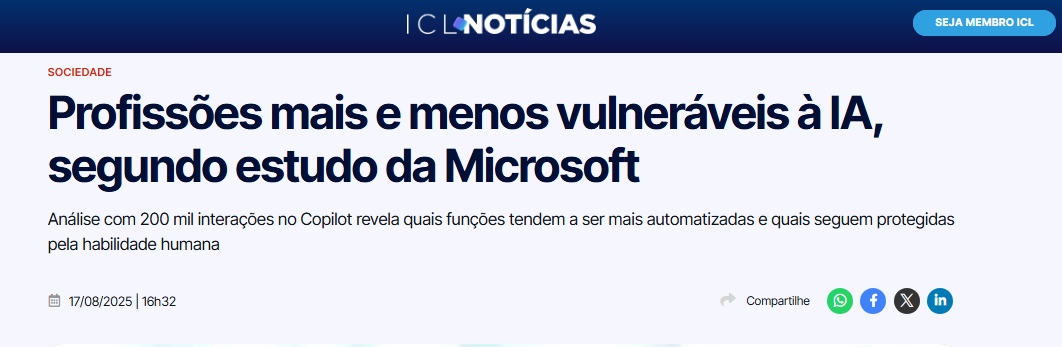
\includegraphics[keepaspectratio]{ICL.png}}

\pandocbounded{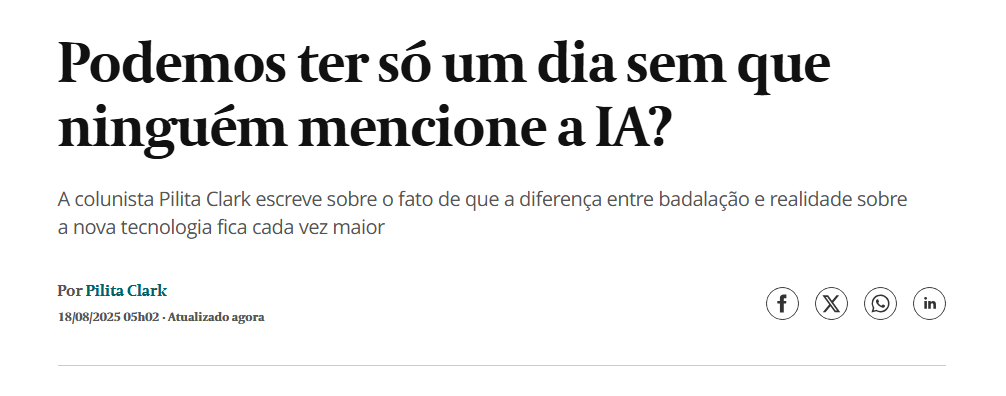
\includegraphics[keepaspectratio]{Valor.png}}

\pandocbounded{
\includegraphics[keepaspectratio]{UOL.png}}

\subsection{Definir a IA}\label{definir-a-ia}

Boden (1996), ``uma classe de tecnologia de alto processamento via
automatização e predição\ldots{} geralmente, com aprendizagem de máquina
e alimentada por grandes volumes de dados''

Para Esposito (2022, xiii),

``A questão não é explicar, mas \textbf{predizer}; não é identificar
relações causais, mas encontrar \textbf{correlações}; não é gerenciar a
incerteza {[}do futuro{]}, mas descobrir quais seriam seus
\textbf{padrões e estruturas}''

\subsection{IA como fenômeno social}\label{ia-como-fenuxf4meno-social-1}

Os sistemas inteligentes estão presentes em várias dimensões da vida
social (educação, mundo do trabalho, cultura etc)

Isso acarreta em um aumento significativo, por parte de países, em
capacitar seus recursos humanos relativos ao campo da IA. \textbf{Mas e
o Brasil nisso tudo?}

\subsection{O que já foi dito a
respeito?}\label{o-que-juxe1-foi-dito-a-respeito}

O primeiro passo de qualquer pesquisa é levantar o que já foi dito a
respeito. No nosso caso, \textbf{o que já foi escrito sobre IA,
tecnologias digitais, conhecimento científico, recursos humanos
qualificados, desenvolvimento econômico?}

Para Pasquinelli (2023), as ciências humanas foram essenciais para
conceber a IA (e.g.~o economista Hayek e suas trocas com engenheiros na
época)

\subsection{Quais as lacunas da
literatura?}\label{quais-as-lacunas-da-literatura}

\begin{itemize}
\tightlist
\item
  Estudos sobre humanidades e ciências sociais aplicadas eram, até
  então, escassos.
\item
  Em geral, os estudos versavam sobre o ``código na cultura'', mas não a
  ``cultura no código'', como Airoldi (2021) aponta
\item
  Com uma exceção (Costa et al. 2021), não havia mapeamentos similares
  sobre a interface entre ``IA'', ``conhecimento científico'' e
  ``Brasil''
\item
  Mapeamentos parecem sub-representar as humanidades.
\end{itemize}

\subsection{Questão sociológica de
pesquisa}\label{questuxe3o-socioluxf3gica-de-pesquisa}

Tendo em vista suprir uma lacuna teórica e abrir novos caminhos
(originais) de pesquisa, nos questionamos:

\textbf{Como os grupos de pesquisa brasileiros em Humanidades e Ciências
Sociais Aplicadas (HCSA) pesquisam Inteligência Artificial e tecnologias
digitais em 2022?}

\subsection{Hipótese}\label{hipuxf3tese}

Geralmente, um levantamento é exploratório. É um ``acelerador de
hipóteses'', à medida que seus resultados permitem abrir novos
horizontes de pesquisa.

Mesmo assim, sempre temos algumas suposições do que vamos encontrar. Uma
das hipóteses centrais era de que \textbf{os grupos de pesquisa são
sub-representados pelos levantamentos já feitos em função de suas
especificidades temáticas}.

\subsection{Objetivos}\label{objetivos}

O objetivo geral era \textbf{mapear} o campo de IA na academia de HCSA
no Brasil.

Para isso, precisaríamos:

\begin{itemize}
\tightlist
\item
  identificar os temas mais investigados pelos grupos pelas suas linhas
  e descrições de pesquisa,
\item
  encontrar padrões na distribuição geográfica, institucional
  (e.g.~categoria administrativa) e social (e.g.~gênero)
\end{itemize}

Em resumo, onde estão os grupos, o que pesquisam, quais são eles e quais
são seus perfis.

\subsection{Referencial empírico}\label{referencial-empuxedrico}

\subsubsection{Unidade de análise}

Nossa população são os grupos de pesquisa registrados no Diretório de
Grupos de Pesquisa do Conselho Nacional de Desenvolvimento Científico e
Tecnológico (DGP/CNPq), cadastrados até outubro de 2022, que tenham a IA
como algum de seus objetos.

Para isso, usamos uma listagem inicial de \textbf{31 descritores} em
português e inglês fornecidos pelo C4AI/USP. Eles foram complementados
com um levantamento bibliográfico (e.g.~``cultura algorítmica'',
``humanidades digitais'' etc).

Isso resultou em um total de 1547 grupos encontrados, retirando
duplicatas. \textbf{Quando olhamos apenas para os HCSA, temos apenas 196
grupos}. Houve uma facilidade do DGP que nos permitiu baixar os grupos
em uma planilha Excel. Com essa listagem, alimentamos o buscador da
raspagem.

\subsubsection{Descritores}

\begin{longtable}[]{@{}
  >{\raggedright\arraybackslash}p{(\linewidth - 6\tabcolsep) * \real{0.5775}}
  >{\raggedright\arraybackslash}p{(\linewidth - 6\tabcolsep) * \real{0.0986}}
  >{\raggedright\arraybackslash}p{(\linewidth - 6\tabcolsep) * \real{0.1690}}
  >{\raggedright\arraybackslash}p{(\linewidth - 6\tabcolsep) * \real{0.1549}}@{}}
\toprule\noalign{}
\begin{minipage}[b]{\linewidth}\raggedright
Descritivo
\end{minipage} & \begin{minipage}[b]{\linewidth}\raggedright
Total
\end{minipage} & \begin{minipage}[b]{\linewidth}\raggedright
Duplicados
\end{minipage} & \begin{minipage}[b]{\linewidth}\raggedright
Resultado
\end{minipage} \\
\midrule\noalign{}
\endhead
\bottomrule\noalign{}
\endlastfoot
inteligência aplicada & 98 & 0 & 98 \\
Inteligência artificial & 765 & 78 & 687 \\
artificial intelligence & 29 & 16 & 13 \\
artificial inteligente & 37 & 37 & 0 \\
Agente de máquina & 251 & 110 & 141 \\
Agente de máquinas & 29 & 29 & 0 \\
agentes inteligentes & 31 & 17 & 14 \\
aprendizado de máquina & 0 & 0 & 0 \\
aprendizado de máquinas & 0 & 0 & 0 \\
aprendizado por máquina (sem resultado) & 0 & 0 & 0 \\
aprendizado profundo & 20 & 17 & 3 \\
aprendizado por reforco & 13 & 11 & 2 \\
automacao inteligente & 31 & 19 & 12 \\
computational intelligence & 4 & 1 & 3 \\
deep learning & 108 & 76 & 32 \\
agents machine learning & 0 & 0 & 0 \\
máquinas de aprendizado & 1 & 1 & 0 \\
redes neurais & 299 & 167 & 132 \\
reinforcement learning & 5 & 5 & 0 \\
robô inteligente & 33 & 20 & 13 \\
robos inteligentes & 3 & 3 & 0 \\
robótica inteligente & 28 & 27 & 1 \\
robótica móvel inteligente & 4 & 4 & 0 \\
sistemas autonomos inteligentes & 5 & 5 & 0 \\
sistemas baseados em aprendizado & 1 & 1 & 0 \\
sistemas especialistas inteligentes & 3 & 3 & 0 \\
sistemas hibridos inteligentes & 2 & 2 & 0 \\
sistema inteligente & 302 & 188 & 114 \\
sistemas inteligentes & 260 & 260 & 0 \\
algorithms & 8 & 4 & 4 \\
algoritmos & 378 & 165 & 213 \\
Humanidades digitais & 49 & 13 & 36 \\
Humanidade digital & 12 & 1 & 11 \\
Natural Language Processing & 7 & 4 & 3 \\
Processamento de Linguagem Natural & 54 & 39 & 15 \\
ética algorítmica & 1 & 0 & 1 \\
engenharia da educação & 7 & 2 & 5 \\
inteligência artificial educação & 22 & 15 & 7 \\
interação humano máquina & 2 & 0 & 2 \\
cultura algorítmica & 2 & 0 & 2 \\
\end{longtable}

\section{Etapa 2. Coleta e produção de
``dados''}\label{etapa-2.-coleta-e-produuxe7uxe3o-de-dados}

\subsection{E agora?}\label{e-agora}

Com a pesquisa desenhada, podemos encontrar maneiras de cumprir com os
objetivos específicos, dando um caminho para verificarmos nossa hipótese
e chegarmos a uma resposta à pergunta de pesquisa.

Feito o levantamento bibliográfico, agora era preciso descobrir os temas
e a composição dos grupos de IA, \textbf{o que demandaria muito tempo da
equipe de pesquisa se fôssemos fazer manualmente.}

Por isso, recorremos à raspagem de dados (ou \emph{web scraping}) do
DGP/CNPq.

\subsection{Web scraping}\label{web-scraping}

\textbf{O que é?} É uma ferramenta computacional que automatiza a
obtenção de dados digitais a partir da estrutura de um site-alvo, que
podem ser redes sociais, repositórios, sites em geral que possuem alguma
estrutura.

Vejamos a estrutura do \href{https://lattes.cnpq.br/web/dgp}{site do
DGP/CNPq}.

\subsection{Web scraping}\label{web-scraping-1}

\textbf{Por quê?} Os objetivos podem ser muitos, mas geralmente usamos
raspagem quando temos um volume muito grande de dados para realizarmos a
pesquisa, tornando-se disponível apenas com o advento do digital e das
ciências sociais computacionais, ver Cordeiro, Gomes, e Waizbort (2023)

\subsection{Ética de pesquisa}\label{uxe9tica-de-pesquisa}

Temos que tomar alguns cuidados quando levamos adiante a raspagem de
dados:

\begin{itemize}
\item
  Atentar-se à Lei Geral de Proteção de Dados (LGDP), especialmente
  \textbf{privacidade}, \textbf{anonimização} e \textbf{armazenamento}
  dos dados.
\item
  Verificar os termos de uso das plataformas raspadas (e.g.~LinkedIn)
\item
  Prestar atenção em possíveis direitos autorais e se há algum risco aos
  envolvidos.
\end{itemize}

É preciso ter \textbf{vigilância epistemológica}.

\subsection{E como fazer?}\label{e-como-fazer}

O primeiro passo é encontrar algum ambiente de programação, as
conhecidas IDEs. O \href{https://colab.google/}{Google Colab} é uma boa
porta de entrada: é usada no navegador, possui suporte do Gemini e é
intuitivo.

Mas há outros: Visual Studio, Anaconda, Spider, RStudio, etc;

\subsection{Antes, veja o site}\label{antes-veja-o-site}

Clique com o botão direito ou aperte F12 para abrir o inspecionar
elemento. Clicando na seta que se encontra no canto superior esquerdo,
que lhe permite investigar qual classe pertence cada objeto do site.

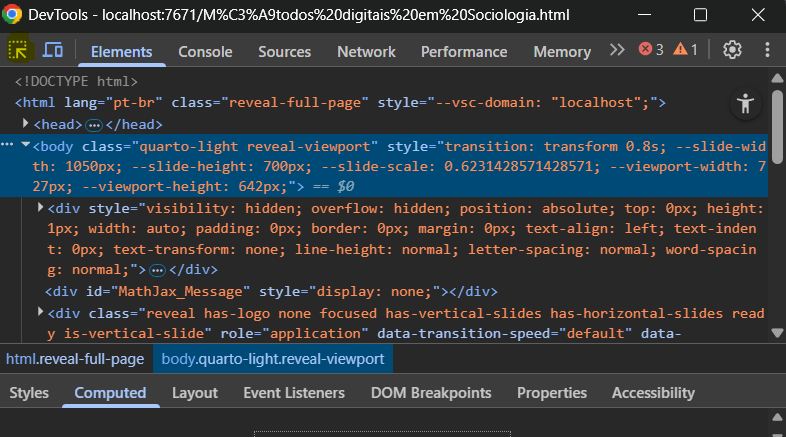
\includegraphics[width=52.08333in,height=\textheight,keepaspectratio]{Inspecionar.png}

\subsection{E como fazer?}\label{e-como-fazer-1}

\subsubsection{Os pacotes}

Há muitas maneiras de se fazer raspagem de dados digitais. H

No nosso caso, recorremos a algumas bibliotecas específicas da linguagem
Python:

\begin{itemize}
\tightlist
\item
  Selenium
\item
  Requests
\item
  BeautifulSoup
\item
  Pandas
\item
  Pickle
\end{itemize}

\subsubsection{Código}

\begin{Shaded}
\begin{Highlighting}[]

\ImportTok{import}\NormalTok{ pytest}
\ImportTok{import}\NormalTok{ time}
\ImportTok{import}\NormalTok{ json}
\ImportTok{from}\NormalTok{ selenium }\ImportTok{import}\NormalTok{ webdriver}
\ImportTok{from}\NormalTok{ selenium.webdriver.common.by }\ImportTok{import}\NormalTok{ By}
\ImportTok{from}\NormalTok{ selenium.webdriver.common.action\_chains }\ImportTok{import}\NormalTok{ ActionChains}
\ImportTok{from}\NormalTok{ selenium.webdriver.support }\ImportTok{import}\NormalTok{ expected\_conditions}
\ImportTok{from}\NormalTok{ selenium.webdriver.support.wait }\ImportTok{import}\NormalTok{ WebDriverWait}
\ImportTok{from}\NormalTok{ selenium.webdriver.common.keys }\ImportTok{import}\NormalTok{ Keys}
\ImportTok{from}\NormalTok{ selenium.webdriver.common.desired\_capabilities }\ImportTok{import}\NormalTok{ DesiredCapabilities}
\ImportTok{import}\NormalTok{ requests}
\ImportTok{import}\NormalTok{ pandas }\ImportTok{as}\NormalTok{ pd}
\ImportTok{from}\NormalTok{ bs4 }\ImportTok{import}\NormalTok{ BeautifulSoup}
\ImportTok{import}\NormalTok{ pickle}
\ImportTok{import}\NormalTok{ warnings}
\NormalTok{warnings.filterwarnings(}\StringTok{"ignore"}\NormalTok{, category}\OperatorTok{=}\PreprocessorTok{UserWarning}\NormalTok{, module}\OperatorTok{=}\StringTok{"bs4"}\NormalTok{)}
\end{Highlighting}
\end{Shaded}

\subsection{O que foi coletado?}\label{o-que-foi-coletado}

\subsubsection{Dados obtidos}

Coletamos a informação sobre

\begin{itemize}
\tightlist
\item
  Instituição e sua respectiva categoria administrativa,
\item
  Localidade,
\item
  Título,
\item
  Nomes de líderes, sub-líderes, pesquisadores e estudantes,
\item
  Área do líder, área e subárea do grupo
\item
  Texto de repercussão (descrição)
\end{itemize}

Com isso, obtemos 7741 linhas de pesquisa, 18181 pesquisadores e 31999
estudantes associados.

\subsubsection{Código}

\begin{Shaded}
\begin{Highlighting}[numbers=left,,]
\CommentTok{\# Função para abrir página em função do tempo de espera}
\KeywordTok{def}\NormalTok{ wait\_for\_window(driver, }\BuiltInTok{vars}\NormalTok{, timeout }\OperatorTok{=} \DecValTok{2}\NormalTok{):}
\NormalTok{    time.sleep(}\BuiltInTok{round}\NormalTok{(timeout }\OperatorTok{/} \DecValTok{1000}\NormalTok{))}
\NormalTok{    wh\_now }\OperatorTok{=}\NormalTok{ driver.window\_handles}
\NormalTok{    wh\_then }\OperatorTok{=} \BuiltInTok{vars}\NormalTok{[}\StringTok{"window\_handles"}\NormalTok{]}
    \ControlFlowTok{if} \BuiltInTok{len}\NormalTok{(wh\_now) }\OperatorTok{\textgreater{}} \BuiltInTok{len}\NormalTok{(wh\_then):}
        \ControlFlowTok{return} \BuiltInTok{set}\NormalTok{(wh\_now).difference(}\BuiltInTok{set}\NormalTok{(wh\_then)).pop()}
    \ControlFlowTok{else}\NormalTok{:}
        \ControlFlowTok{return} \StringTok{\textquotesingle{}Não abriu a página\textquotesingle{}}
    
\CommentTok{\# Cria uma lista e permite inserir os grupos baixados da planilha}
\NormalTok{grupos }\OperatorTok{=}\NormalTok{ [] }\CommentTok{\# Insira aqui os nomes dos grupo}

\CommentTok{\# Automação de raspagem:}
\NormalTok{output }\OperatorTok{=}\NormalTok{ []   }

\CommentTok{\# Selenium em ação}
\ControlFlowTok{for}\NormalTok{ g }\KeywordTok{in}\NormalTok{ grupos:                }\CommentTok{\# Cria um loop}
\NormalTok{    driver }\OperatorTok{=}\NormalTok{ webdriver.Chrome() }\CommentTok{\# Usa Selenium para acoplar ao Google Chrome}
\NormalTok{    driver.implicitly\_wait(}\DecValTok{10}\NormalTok{)  }\CommentTok{\# Tempo de espera}
    \BuiltInTok{vars} \OperatorTok{=}\NormalTok{ \{\}                   }\CommentTok{\# Cria um dicionário vazio}
\NormalTok{    driver.get(}\StringTok{"http://dgp.cnpq.br/dgp/faces/consulta/consulta\_parametrizada.jsf"}\NormalTok{)}
\NormalTok{    driver.find\_element(By.ID, }\StringTok{"idFormConsultaParametrizada:idTextoFiltro"}\NormalTok{).click() }\CommentTok{\# Clica!}
\NormalTok{    driver.find\_element(By.ID, }\StringTok{"idFormConsultaParametrizada:idTextoFiltro"}\NormalTok{).send\_keys(g)}
\NormalTok{    driver.find\_element(By.ID, }\StringTok{"idFormConsultaParametrizada:campos:1"}\NormalTok{).click()}
\NormalTok{    driver.find\_element(By.ID, }\StringTok{"idFormConsultaParametrizada:campos:2"}\NormalTok{).click()}
\NormalTok{    driver.find\_element(By.CSS\_SELECTOR, }\StringTok{"\#idFormConsultaParametrizada}\CharTok{\textbackslash{}\textbackslash{}}\StringTok{3AidPesquisar \textgreater{} .ui{-}button{-}text"}\NormalTok{).click()}
    \BuiltInTok{vars}\NormalTok{[}\StringTok{"window\_handles"}\NormalTok{] }\OperatorTok{=}\NormalTok{ driver.window\_handles}

\NormalTok{    driver.find\_element(By.ID, }\StringTok{"idFormConsultaParametrizada:resultadoDataList:0:idBtnVisualizarEspelhoGrupo"}\NormalTok{).click()}
    \BuiltInTok{vars}\NormalTok{[}\StringTok{"win3115"}\NormalTok{] }\OperatorTok{=}\NormalTok{ wait\_for\_window(driver, }\BuiltInTok{vars}\NormalTok{, timeout }\OperatorTok{=} \DecValTok{3000}\NormalTok{)}
\NormalTok{    driver.switch\_to.window(}\BuiltInTok{vars}\NormalTok{[}\StringTok{"win3115"}\NormalTok{])}
\NormalTok{    driver.execute\_script(}\StringTok{"window.scrollTo(0,306)"}\NormalTok{)}


    \CommentTok{\# Raspagem de dados com BeatifulSoup:}
\NormalTok{    response }\OperatorTok{=}\NormalTok{ requests.get(driver.current\_url)}
\NormalTok{    content }\OperatorTok{=}\NormalTok{ response.content}
\NormalTok{    site }\OperatorTok{=}\NormalTok{ BeautifulSoup(content, }\StringTok{\textquotesingle{}html.parser\textquotesingle{}}\NormalTok{)}

    \ControlFlowTok{try}\NormalTok{:}
\NormalTok{        repercussao }\OperatorTok{=}\NormalTok{ site.find(}\StringTok{\textquotesingle{}div\textquotesingle{}}\NormalTok{, }\BuiltInTok{id}\OperatorTok{=}\StringTok{"repercussao"}\NormalTok{)}
\NormalTok{        paragraph }\OperatorTok{=}\NormalTok{ repercussao.find(}\StringTok{\textquotesingle{}p\textquotesingle{}}\NormalTok{)}
        \ControlFlowTok{if}\NormalTok{ paragraph:}
\NormalTok{            repercussao\_text }\OperatorTok{=}\NormalTok{ paragraph.get\_text()}
            \BuiltInTok{print}\NormalTok{(repercussao\_text)}
        \ControlFlowTok{else}\NormalTok{:}
            \BuiltInTok{print}\NormalTok{(}\StringTok{\textquotesingle{}Não há texto de repercussão\textquotesingle{}}\NormalTok{)}
    \ControlFlowTok{except}\NormalTok{:}
        \BuiltInTok{print}\NormalTok{(}\StringTok{\textquotesingle{}Erro ao obter texto de repercussão\textquotesingle{}}\NormalTok{)}
             
\NormalTok{    lista }\OperatorTok{=}\NormalTok{ []}
\NormalTok{    lista.append(g)}
\NormalTok{    lista.append(pd.read\_html(response.text))}
\NormalTok{    driver.quit()}
    
\NormalTok{    output.append(lista)}

\ControlFlowTok{if}\NormalTok{ repercussao\_text:}
    \ControlFlowTok{with} \BuiltInTok{open}\NormalTok{(}\StringTok{\textquotesingle{}repercussaotesteout.txt\textquotesingle{}}\NormalTok{, }\StringTok{\textquotesingle{}w\textquotesingle{}}\NormalTok{, encoding}\OperatorTok{=}\StringTok{\textquotesingle{}utf{-}8\textquotesingle{}}\NormalTok{) }\ImportTok{as}\NormalTok{ arquivo\_texto:}
\NormalTok{        arquivo\_texto.write(}\StringTok{"texto de repercussão: "}\NormalTok{)}
\NormalTok{        arquivo\_texto.write(repercussao\_text)}
\NormalTok{        arquivo\_texto.write(}\StringTok{"}\CharTok{\textbackslash{}n}\StringTok{"}\NormalTok{)}
    
\ControlFlowTok{with} \BuiltInTok{open}\NormalTok{(}\StringTok{\textquotesingle{}outputtesteout.pkl\textquotesingle{}}\NormalTok{, }\StringTok{\textquotesingle{}wb\textquotesingle{}}\NormalTok{) }\ImportTok{as}\NormalTok{ arquivo:}
\NormalTok{    pickle.dump(output, arquivo)}

\NormalTok{output}
\end{Highlighting}
\end{Shaded}

\subsubsection{Output}

\begin{verbatim}
O Grupo de Pesquisa "Inteligência Artificial e Sociedade" tem sua base no Centro for Artificial Intelligence (C4AI) da Universidade de São Paulo. O Grupo está voltado para a pesquisa na área de humanidades, com estudos orientados para as políticas públicas em países emergentes. Temas como as Transformações do Trabalho, Emprego, Novas Tecnologias e Competências, Regulação, Ética, Privacidade, Ética Corporativa, Impactos sociais de técnicas Biométricas, Informação e Desinformação, Democracia, Cidades Inteligentes e Relações Homem-Robô.Dada sua característica multidisciplinar e multiinstitucional, Grupo abriga pesquisadores da Sociologia, Ciência Política, Economia, Psicologia, Computação, Medicina, Direito, Comunicação, Robótica. Os trabalhos de pesquisa estão voltados para consolidar a Inteligência Artificial no Brasil e ampliar os laços com centros internacionais relevantes. Como parte do C4AI, o Grupo buscará de modo permanente a sinergia com todas as áreas avançadas da IA. 
            
[['Inteligência Artificial e Sociedade',
  [             Rede de pesquisa                Website/Blog
   0  Nenhum registro adicionado  Nenhum registro adicionado,
                              Nome da linha de pesquisa  \
   0  Comunicação e sociabilidade - Jornalismo, proc...   
   1  Implicações éticas, sociais e políticas dos si...   
   2                                    Robótica Social   
   3                         Transformações do Trabalho   
   4           Ética, Direito e Inteligência Artificial   
   
      Quantidade de Estudantes  Quantidade de Pesquisadores  \
   0                         1                            2   
   1                         4                            3   
   2                         3                            2   
   3                         8                            2   
   4                         0                            1   
   
                                                  Ações  
   0  Visualizar espelho da linha de pesquisa$(funct...  
   1  Visualizar espelho da linha de pesquisa$(funct...  
   2  Visualizar espelho da linha de pesquisa$(funct...  
   3  Visualizar espelho da linha de pesquisa$(funct...  
   4  Visualizar espelho da linha de pesquisa$(funct...  ,
                            Pesquisadores Titulação máxima Data inclusão  \
   0                 Alvaro Augusto Comin        Doutorado    07/02/2022   
   1  Cristina Godoy Bernardo de Oliveira        Doutorado    07/02/2022   
   2                        Eugênio Bucci        Doutorado    07/02/2022   
   3          Glauco Antonio Truzzi Arbix        Doutorado    23/07/2020   
   4              João Paulo Cândia Veiga        Doutorado    07/02/2022   
   5             Magaly Parreira do Prado        Doutorado    09/02/2022   
   6                    Marcelo Fantinato        Doutorado    23/02/2022   
   7     Murillo Marschner Alves de Brito        Doutorado    09/02/2022   
   8               Sarajane Marques Peres        Doutorado    07/02/2022   
   
                                                  Ações  
   0  Visualizar Currículo Lattes$(function(){PrimeF...  
   1  Visualizar Currículo Lattes$(function(){PrimeF...  
   2  Visualizar Currículo Lattes$(function(){PrimeF...  
   3  Visualizar Currículo Lattes$(function(){PrimeF...  
   4  Visualizar Currículo Lattes$(function(){PrimeF...  
   5  Visualizar Currículo Lattes$(function(){PrimeF...  
   6  Visualizar Currículo Lattes$(function(){PrimeF...  
   7  Visualizar Currículo Lattes$(function(){PrimeF...  
   8  Visualizar Currículo Lattes$(function(){PrimeF...  ,
                               Estudantes          Nível de Treinamento  \
   0                          André Scerb                      Mestrado   
   1          Bernardo Martinho Ballardin                      Mestrado   
   2              Bruno Sanchez de Araujo                     Doutorado   
   3      Diana Veronica Portugal Churata  Não há formação em andamento   
   4              Eliana Sanches de Frias                      Mestrado   
   5          Flora Bueno de Araujo Ariza                     Graduação   
   6              Gabriela Soares Schmidt                      Mestrado   
   7           Guilherme Olímpio Fagundes                     Graduação   
   8          Jonatas Mendonça dos Santos                     Doutorado   
   9                 Laura Simões Camargo  Não há formação em andamento   
   10         Marcus Vinicius Santos Repa                     Doutorado   
   11         Otávio De Paula Albuquerque                     Doutorado   
   12  Rodrigo Brandão de Andrade e Silva                     Doutorado   
   13         Thiago de Oliveira Meireles                     Doutorado   
   
      Data inclusão                                              Ações  
   0     24/03/2022  Visualizar Currículo Lattes$(function(){PrimeF...  
   1     24/03/2022  Visualizar Currículo Lattes$(function(){PrimeF...  
   2     23/02/2022  Visualizar Currículo Lattes$(function(){PrimeF...  
   3     23/02/2022  Visualizar Currículo Lattes$(function(){PrimeF...  
   4     16/02/2022  Visualizar Currículo Lattes$(function(){PrimeF...  
   5     24/03/2022  Visualizar Currículo Lattes$(function(){PrimeF...  
   6     24/03/2022  Visualizar Currículo Lattes$(function(){PrimeF...  
   7     24/03/2022  Visualizar Currículo Lattes$(function(){PrimeF...  
   8     07/02/2022  Visualizar Currículo Lattes$(function(){PrimeF...  
   9     07/02/2022  Visualizar Currículo Lattes$(function(){PrimeF...  
   10    24/03/2022  Visualizar Currículo Lattes$(function(){PrimeF...  
   11    23/02/2022  Visualizar Currículo Lattes$(function(){PrimeF...  
   12    07/02/2022  Visualizar Currículo Lattes$(function(){PrimeF...  
   13    09/02/2022  Visualizar Currículo Lattes$(function(){PrimeF...  ,
                        Técnicos          Formação acadêmica  \
   0  Nenhum registro adicionado  Nenhum registro adicionado   
   
                   Data inclusão                       Ações  
   0  Nenhum registro adicionado  Nenhum registro adicionado  ,
      Colaboradores estrangeiros                        País  \
   0  Nenhum registro adicionado  Nenhum registro adicionado   
   
                   Data inclusão                       Ações  
   0  Nenhum registro adicionado  Nenhum registro adicionado  ,
                   Pesquisadores Período de participação no grupo  \
   0  Nenhum registro adicionado       Nenhum registro adicionado   
   
                           Ações  
   0  Nenhum registro adicionado  ,
                      Estudantes Período de participação no grupo  \
   0  Nenhum registro adicionado       Nenhum registro adicionado   
   
                           Ações  
   0  Nenhum registro adicionado  ,
                          Perfil                 Data início  \
   0  Nenhum registro adicionado  Nenhum registro adicionado   
   
                        Data fim  
   0  Nenhum registro adicionado  ,
     Nome da Instituição Parceira                       Sigla  \
   0   Nenhum registro adicionado  Nenhum registro adicionado   
   
                              UF                       Ações  
   0  Nenhum registro adicionado  Nenhum registro adicionado  ,
     Formação acadêmica  Pesquisadores  Estudantes  Técnicos  \
   0          Doutorado              9           6         0   
   1           Mestrado              0           4         0   
   2          Graduação              0           1         0   
   3             Outros              0           3         0   
   
      Colaboradores estrangeiros  Total  
   0                           0     15  
   1                           0      4  
   2                           0      1  
   3                           0      3  ,
                    Equipamentos                       Ações
   0  Nenhum registro adicionado  Nenhum registro adicionado,
                       Softwares                       Ações
   0  Nenhum registro adicionado  Nenhum registro adicionado,
      Unnamed: 0                       Itens
   0         NaN               Identificação
   1         NaN                    Endereço
   2         NaN  Repercussões dos trabalhos
   3         NaN          Linhas de pesquisa
   4         NaN            Recursos humanos
   5         NaN           Indicadores de RH]]]
\end{verbatim}

\subsection{Raspadores disponíveis}\label{raspadores-disponuxedveis}

Há raspadores disponíveis quase prontos para usuários poderem usar.

Vale a pena procurar pelo GitHub. Um deles é o raspador do portal de
notícias do G1, pelo colega uspiano José A. Soares de Oliveira
(hermengardo, no
\href{https://github.com/hermengardo/G1_news_scraper/blob/main}{GitHub})

Também existe opções para
\href{https://github.com/vladkens/twscrape}{Twitter/X}, TikTok,
Instagram, YouTube dentre outros, ver Omena et al. (2024).

\subsection{Estruturando o banco de
dados}\label{estruturando-o-banco-de-dados}

É comum que o banco venha bagunçado. Mas não desanime! A raspagem requer
que a pessoa que esteja raspando tenha a paciência de fazer várias
iterações (idas e vindas) com o código, sempre melhorando-o.

No nosso caso, tivemos muitas duplicatas ou trocas de valores das
variáveis (e.g.~onde deveria estar ``nome do grupo'' vinha com o nome do
pesquisador). Correções serão sempre necessárias.

\section{Etapa 3. Análise e sistematização dos
dados}\label{etapa-3.-anuxe1lise-e-sistematizauxe7uxe3o-dos-dados}

\subsection{Tratamento do banco de
dados}\label{tratamento-do-banco-de-dados}

Depois de obter o banco, tivemos o trabalho de verificar
inconsistências, corrigir manualmente eventuais erros, bem como
condicioná-la para aplicar os instrumentos de análise, como a modelagem
de tópicos via Python/Colab e a análise textual via Iramuteq.

Alguns dos procedimentos foram a \textbf{tokenização} e a
\textbf{lematização}, usando o ChatGPT + Spacy e verificando se não
houve alucinação.

\subsection{Classificando as
observações}\label{classificando-as-observauxe7uxf5es}

Usando a tipologia de Liu (2021), duplas de pesquisadores classificaram
se os grupos pesquisavam

\begin{itemize}
\tightlist
\item
  IA como objeto (\emph{n} = 55)
\item
  IA como método (\emph{n} = 42)
\item
  Ambos (\emph{n} = 33)
\item
  Tecnologias digitais (\emph{n} = 66)
\end{itemize}

Isso é uma tarefa que, com aprendizagem de máquina, poderia ser feita.
Mas por serem apenas 196 grupos para 6 estudantes de IC, a classificação
foi manual.

\subsection{Banco de dados tratado}\label{banco-de-dados-tratado}

\pandocbounded{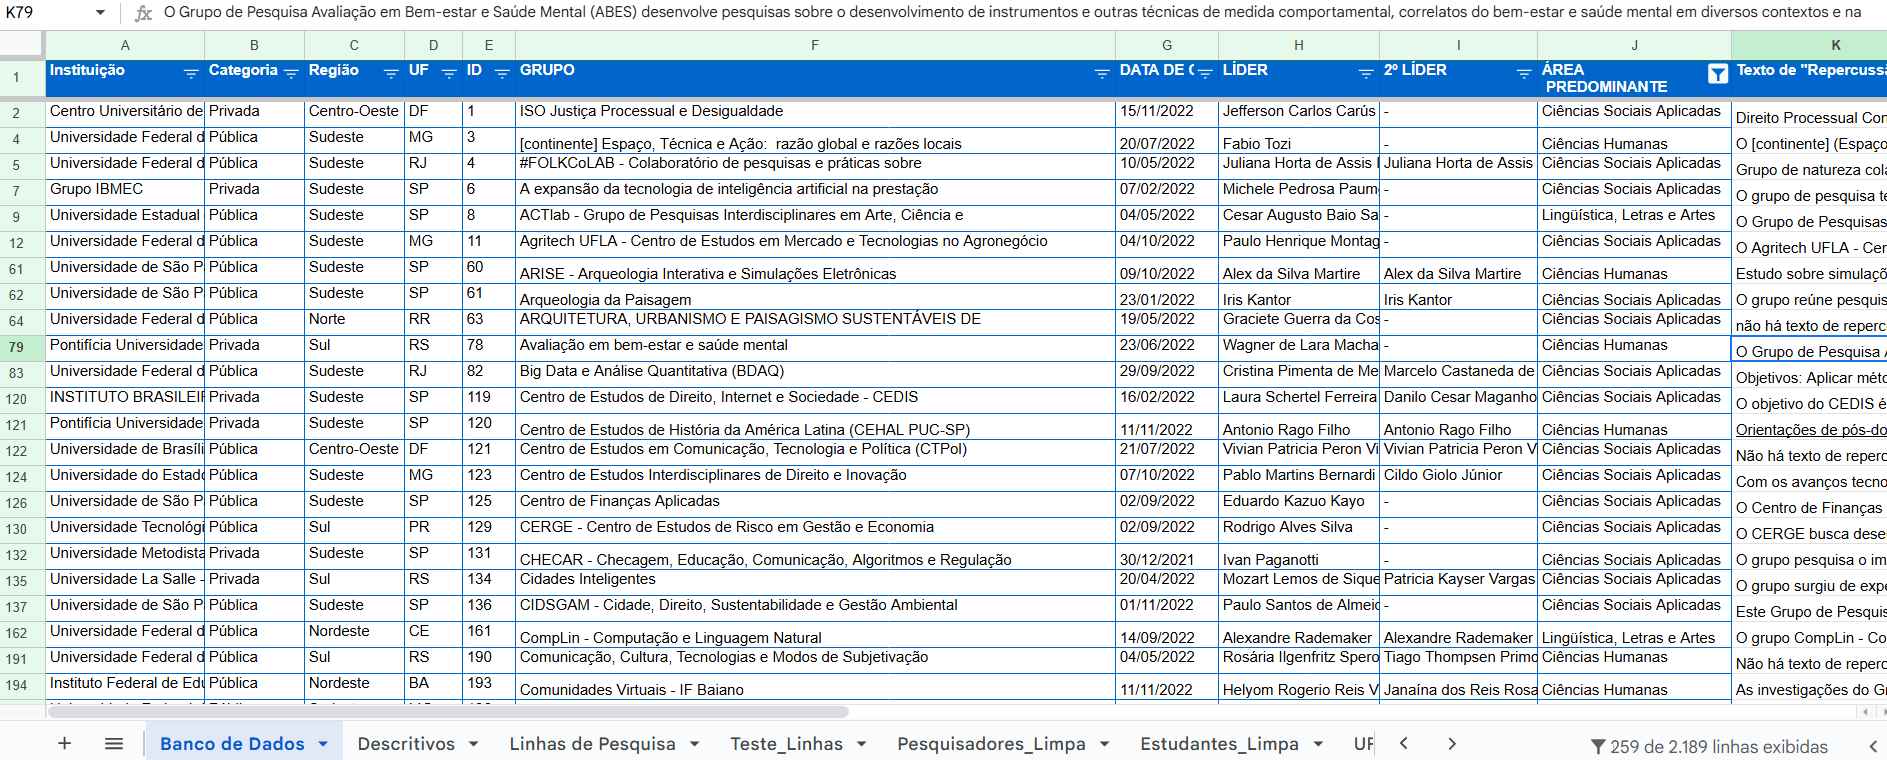
\includegraphics[keepaspectratio]{Banco.png}}

\subsection{Modelagem de tópicos}\label{modelagem-de-tuxf3picos}

\subsubsection{O que é?}

Os métodos digitais não foram unicamente usados para a coleta, mas
também para a análise.

Recorremos à \textbf{modelagem de tópicos} para explorar os tópicos mais
presentes e similares dos repertórios e linhas de pesquisa. A ideia é
verificar como se formam \emph{clusters} de grupos a partir do que
pesquisam.

Esse instrumento de Processamento de Linguagem Natural (PLN) possui
diferentes modelos. O mais comum é o LDA, mas usamos CorEx. Hoje, há
outros modelos, como a modelagem estrutural de tópicos (STM), que possui
maior facilidade para analisar grandes volumes de dados.

\subsubsection{Código}

\begin{Shaded}
\begin{Highlighting}[]

\CommentTok{\# Pacotes}
\ImportTok{import}\NormalTok{ nltk}
\ImportTok{import}\NormalTok{ pandas }\ImportTok{as}\NormalTok{ pd}

\ImportTok{from}\NormalTok{ corextopic }\ImportTok{import}\NormalTok{ corextopic }\ImportTok{as}\NormalTok{ ct}

\ImportTok{from}\NormalTok{ sklearn.feature\_extraction.text }\ImportTok{import}\NormalTok{ TfidfVectorizer}
\ImportTok{from}\NormalTok{ sklearn.feature\_extraction.text }\ImportTok{import}\NormalTok{ CountVectorizer}

\CommentTok{\# Caminho da planilha (abaixo, o exemplo)}
\NormalTok{caminho }\OperatorTok{=} \StringTok{\textquotesingle{}\textquotesingle{}} 

\CommentTok{\# caminho = \textquotesingle{}C://Users//Gloria//Documents//1 USP//IC//Modelagem//modelagem\_class\_objeto.xlsx\textquotesingle{}}

\NormalTok{dataframe }\OperatorTok{=}\NormalTok{ pd.read\_excel(caminho)}
\CommentTok{\#Colunas para textos de repercussão}
\CommentTok{\#nomes\_colunas = ["Instituição", "Categoria", "Região", "UF", "ID", "Grupo", "Data\_Criacao", "Líder", "2º\_Líder", "Subarea\_grupo", "Área\_líder", "Repercussao" ]}

\CommentTok{\#Coluna para linhas de pesquisa}
\CommentTok{\#nomes\_colunas = ["ID", "Categoria", "Grupo", "Área", "ID\_Linha", "Linha","Q\_Estudantes", "Q\_Pesquisadores", "Subarea\_Grupo", "Subarea\_Lider", "Avaliação"]}

\NormalTok{nomes\_colunas }\OperatorTok{=}\NormalTok{ [}\StringTok{"ID"}\NormalTok{, }\StringTok{"Grupo"}\NormalTok{, }\StringTok{"Linha\_"}\NormalTok{, }\StringTok{"área"}\NormalTok{, }\StringTok{"class"}\NormalTok{, }\StringTok{"Lematização"}\NormalTok{, }\StringTok{"Corpus\_FF"}\NormalTok{, }\StringTok{"Linha"}\NormalTok{]}

\NormalTok{df }\OperatorTok{=}\NormalTok{ pd.read\_excel(caminho, names}\OperatorTok{=}\NormalTok{nomes\_colunas)}

\CommentTok{\#dataframe = dataframe.loc[dataframe["Subarea\_Grupo"] == \textquotesingle{}Administração\textquotesingle{}]}

\NormalTok{df}

\NormalTok{vectorizer }\OperatorTok{=}\NormalTok{ TfidfVectorizer(}
\NormalTok{    max\_df}\OperatorTok{=}\FloatTok{.5}\NormalTok{,}
\NormalTok{    min\_df}\OperatorTok{=}\DecValTok{2}\NormalTok{,}
\NormalTok{    max\_features}\OperatorTok{=}\VariableTok{None}\NormalTok{,}
\NormalTok{    ngram\_range}\OperatorTok{=}\NormalTok{(}\DecValTok{1}\NormalTok{, }\DecValTok{2}\NormalTok{),}
\NormalTok{    norm}\OperatorTok{=}\VariableTok{None}\NormalTok{,}
\NormalTok{    binary}\OperatorTok{=}\VariableTok{True}\NormalTok{,}
\NormalTok{    use\_idf}\OperatorTok{=}\VariableTok{False}\NormalTok{,}
\NormalTok{    sublinear\_tf}\OperatorTok{=}\VariableTok{False}
\NormalTok{)}
\NormalTok{vectorizer }\OperatorTok{=}\NormalTok{ vectorizer.fit(df[}\StringTok{\textquotesingle{}Linha\textquotesingle{}}\NormalTok{])}
\NormalTok{tfidf }\OperatorTok{=}\NormalTok{ vectorizer.transform(df[}\StringTok{\textquotesingle{}Linha\textquotesingle{}}\NormalTok{])}
\NormalTok{vocab }\OperatorTok{=}\NormalTok{ vectorizer.get\_feature\_names\_out()}
\BuiltInTok{print}\NormalTok{(}\BuiltInTok{len}\NormalTok{(vocab))}

\KeywordTok{def}\NormalTok{ calcular\_termos\_mais\_comuns(dataframe, coluna, quantidade\_top\_n}\OperatorTok{=}\DecValTok{20}\NormalTok{):}
\NormalTok{    textos\_concatenados }\OperatorTok{=} \StringTok{\textquotesingle{} \textquotesingle{}}\NormalTok{.join(dataframe[coluna].astype(}\BuiltInTok{str}\NormalTok{).tolist())}
\NormalTok{    vectorizer }\OperatorTok{=}\NormalTok{ CountVectorizer()}
\NormalTok{    matriz\_contagem }\OperatorTok{=}\NormalTok{ vectorizer.fit\_transform([textos\_concatenados])}

\NormalTok{    termos }\OperatorTok{=}\NormalTok{ vectorizer.get\_feature\_names\_out()}
\NormalTok{    contagens }\OperatorTok{=}\NormalTok{ matriz\_contagem.toarray().flatten()}

\NormalTok{    df\_termos }\OperatorTok{=}\NormalTok{ pd.DataFrame(\{}\StringTok{\textquotesingle{}Termo\textquotesingle{}}\NormalTok{: termos, }\StringTok{\textquotesingle{}Contagem\textquotesingle{}}\NormalTok{: contagens\})}
\NormalTok{    termos\_mais\_comuns }\OperatorTok{=}\NormalTok{ df\_termos.sort\_values(by}\OperatorTok{=}\StringTok{\textquotesingle{}Contagem\textquotesingle{}}\NormalTok{, ascending}\OperatorTok{=}\VariableTok{False}\NormalTok{).head(quantidade\_top\_n)}

    \ControlFlowTok{return}\NormalTok{ termos\_mais\_comuns}


\NormalTok{termos\_comuns }\OperatorTok{=}\NormalTok{ calcular\_termos\_mais\_comuns(df, }\StringTok{\textquotesingle{}Linha\textquotesingle{}}\NormalTok{)}
\BuiltInTok{print}\NormalTok{(termos\_comuns)}

\CommentTok{\# Definir âncoras}
\NormalTok{anchors }\OperatorTok{=}\NormalTok{ []}
\NormalTok{model }\OperatorTok{=}\NormalTok{ ct.Corex(n\_hidden}\OperatorTok{=}\DecValTok{5}\NormalTok{, seed}\OperatorTok{=}\DecValTok{42}\NormalTok{)}
\NormalTok{model }\OperatorTok{=}\NormalTok{ model.fit(}
\NormalTok{    tfidf,}
\NormalTok{    words}\OperatorTok{=}\NormalTok{vocab}
\NormalTok{)}

\CommentTok{\# Modelagem sem âncoras.}
\ControlFlowTok{for}\NormalTok{ i, topic\_ngrams }\KeywordTok{in} \BuiltInTok{enumerate}\NormalTok{(model.get\_topics(n\_words}\OperatorTok{=}\DecValTok{10}\NormalTok{)):}
\NormalTok{    topic\_ngrams }\OperatorTok{=}\NormalTok{ [ngram[}\DecValTok{0}\NormalTok{] }\ControlFlowTok{for}\NormalTok{ ngram }\KeywordTok{in}\NormalTok{ topic\_ngrams }\ControlFlowTok{if}\NormalTok{ ngram[}\DecValTok{1}\NormalTok{] }\OperatorTok{\textgreater{}} \DecValTok{0}\NormalTok{]}
    \BuiltInTok{print}\NormalTok{(}\StringTok{"Tópico \#}\SpecialCharTok{\{\}}\StringTok{: }\SpecialCharTok{\{\}}\StringTok{"}\NormalTok{.}\BuiltInTok{format}\NormalTok{(i}\OperatorTok{+}\DecValTok{1}\NormalTok{, }\StringTok{", "}\NormalTok{.join(topic\_ngrams)))}
    
\NormalTok{anchors }\OperatorTok{=}\NormalTok{ [}
\NormalTok{    [}\StringTok{"desenvolvimento"}\NormalTok{, }\StringTok{"inovação"}\NormalTok{],}
\NormalTok{    [}\StringTok{"economia"}\NormalTok{, }\StringTok{"trabalho"}\NormalTok{],}
\NormalTok{    [}\StringTok{"instutuição"}\NormalTok{],}
\NormalTok{    [}\StringTok{"governo"}\NormalTok{, }\StringTok{"politica\_publica"}\NormalTok{],}
\NormalTok{    [}\StringTok{"educação"}\NormalTok{, }\StringTok{"ensino"}\NormalTok{],}
\NormalTok{]}

\NormalTok{anchors }\OperatorTok{=}\NormalTok{ [}
\NormalTok{    [a }\ControlFlowTok{for}\NormalTok{ a }\KeywordTok{in}\NormalTok{ topic }\ControlFlowTok{if}\NormalTok{ a }\KeywordTok{in}\NormalTok{ vocab]}
    \ControlFlowTok{for}\NormalTok{ topic }\KeywordTok{in}\NormalTok{ anchors}
\NormalTok{]}

\NormalTok{model }\OperatorTok{=}\NormalTok{ ct.Corex(n\_hidden}\OperatorTok{=}\DecValTok{5}\NormalTok{, seed}\OperatorTok{=}\DecValTok{42}\NormalTok{)}
\NormalTok{model }\OperatorTok{=}\NormalTok{ model.fit(}
\NormalTok{    tfidf,}
\NormalTok{    words}\OperatorTok{=}\NormalTok{vocab,}
\NormalTok{    anchors}\OperatorTok{=}\NormalTok{anchors,}
\NormalTok{    anchor\_strength}\OperatorTok{=}\DecValTok{3}
    
\CommentTok{\# Novamente, mas com âncoras agora}
\ControlFlowTok{for}\NormalTok{ i, topic\_ngrams }\KeywordTok{in} \BuiltInTok{enumerate}\NormalTok{(model.get\_topics(n\_words}\OperatorTok{=}\DecValTok{20}\NormalTok{)):}
\NormalTok{    topic\_ngrams }\OperatorTok{=}\NormalTok{ [ngram[}\DecValTok{0}\NormalTok{] }\ControlFlowTok{for}\NormalTok{ ngram }\KeywordTok{in}\NormalTok{ topic\_ngrams }\ControlFlowTok{if}\NormalTok{ ngram[}\DecValTok{1}\NormalTok{] }\OperatorTok{\textgreater{}} \DecValTok{0}\NormalTok{]}
    \BuiltInTok{print}\NormalTok{(}\StringTok{"Tópico \#}\SpecialCharTok{\{\}}\StringTok{: }\SpecialCharTok{\{\}}\StringTok{"}\NormalTok{.}\BuiltInTok{format}\NormalTok{(i}\OperatorTok{+}\DecValTok{1}\NormalTok{, }\StringTok{", "}\NormalTok{.join(topic\_ngrams)))}
\end{Highlighting}
\end{Shaded}

\subsection{Iramuteq}\label{iramuteq}

Além da modelagem de tópicos, também mobilizamos o software francês
\emph{Interface de R pour les Analyses Multidimensionnelles de Textes et
de Questionnaires} (\textbf{Iramuteq}).

Essa ferramenta computacional, que não possui uso de IA, permite se
aprofundar em algumas análises textuais, como veremos a seguir.

O problema é que ele \emph{não} é um software intuitivo e é de difícil
manipulação. Também requer uma versão desatualizada do R para funcionar.

\subsection{Iramuteq}\label{iramuteq-1}

\subsubsection{Como usar?}

O \emph{corpus} textual, como os textos de repertórios ou linhas de
pesquisa, precisa ser organizado de uma forma específica:

Quatro astericos (****) seguido dos valores de cada variável
(público/privado, áreas, etc)

\subsubsection{Exemplo com linhas de pesquisa}

\pandocbounded{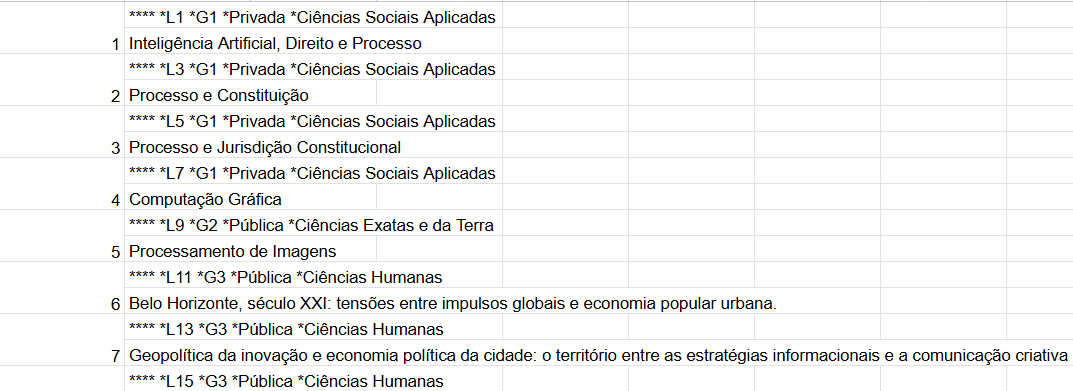
\includegraphics[keepaspectratio]{IRAMUTEQ.png}}

\section{Etapa 4. Interpretação dos
resultados}\label{etapa-4.-interpretauxe7uxe3o-dos-resultados}

\subsection{Panorama dos grupos de pesquisa sobre
IA}\label{panorama-dos-grupos-de-pesquisa-sobre-ia}

\begin{longtable}[]{@{}
  >{\raggedright\arraybackslash}p{(\linewidth - 0\tabcolsep) * \real{1.0000}}@{}}
\toprule\noalign{}
\begin{minipage}[b]{\linewidth}\raggedright
Tópicos e termos associados
\end{minipage} \\
\midrule\noalign{}
\endhead
\bottomrule\noalign{}
\endlastfoot
\textbf{Tópico 1. Inovação e desenvolvimento}: sustentável,
empreendedorismo, propriedade intelectual, saúde, indústria, ética,
comunicação \\
\textbf{Tópico 2. Economia e trabalho}: instituição, globalização,
desenvolvimento, vigilância, governança, decolonial, startup \\
\textbf{Tópico 3. Governo e políticas públicas}: economia,
transparência, dados abertos, regulação, controle, gestão \\
\textbf{Tópico 4. Educação e ensino}: educação, ensino, matemática \\
\textbf{Tópico 5. Meio ambiente}: socioambiental, agronegócio, político,
ética, conflito, transculturalidade, mercado \\
\end{longtable}

\subsection{Mapas\ldots{}}\label{mapas}

\subsubsection{Plotagem}

\pandocbounded{\includegraphics[keepaspectratio]{distribuicao_grupos_pesquisa_Ciências_Humanas_brasil.png}}

\pandocbounded{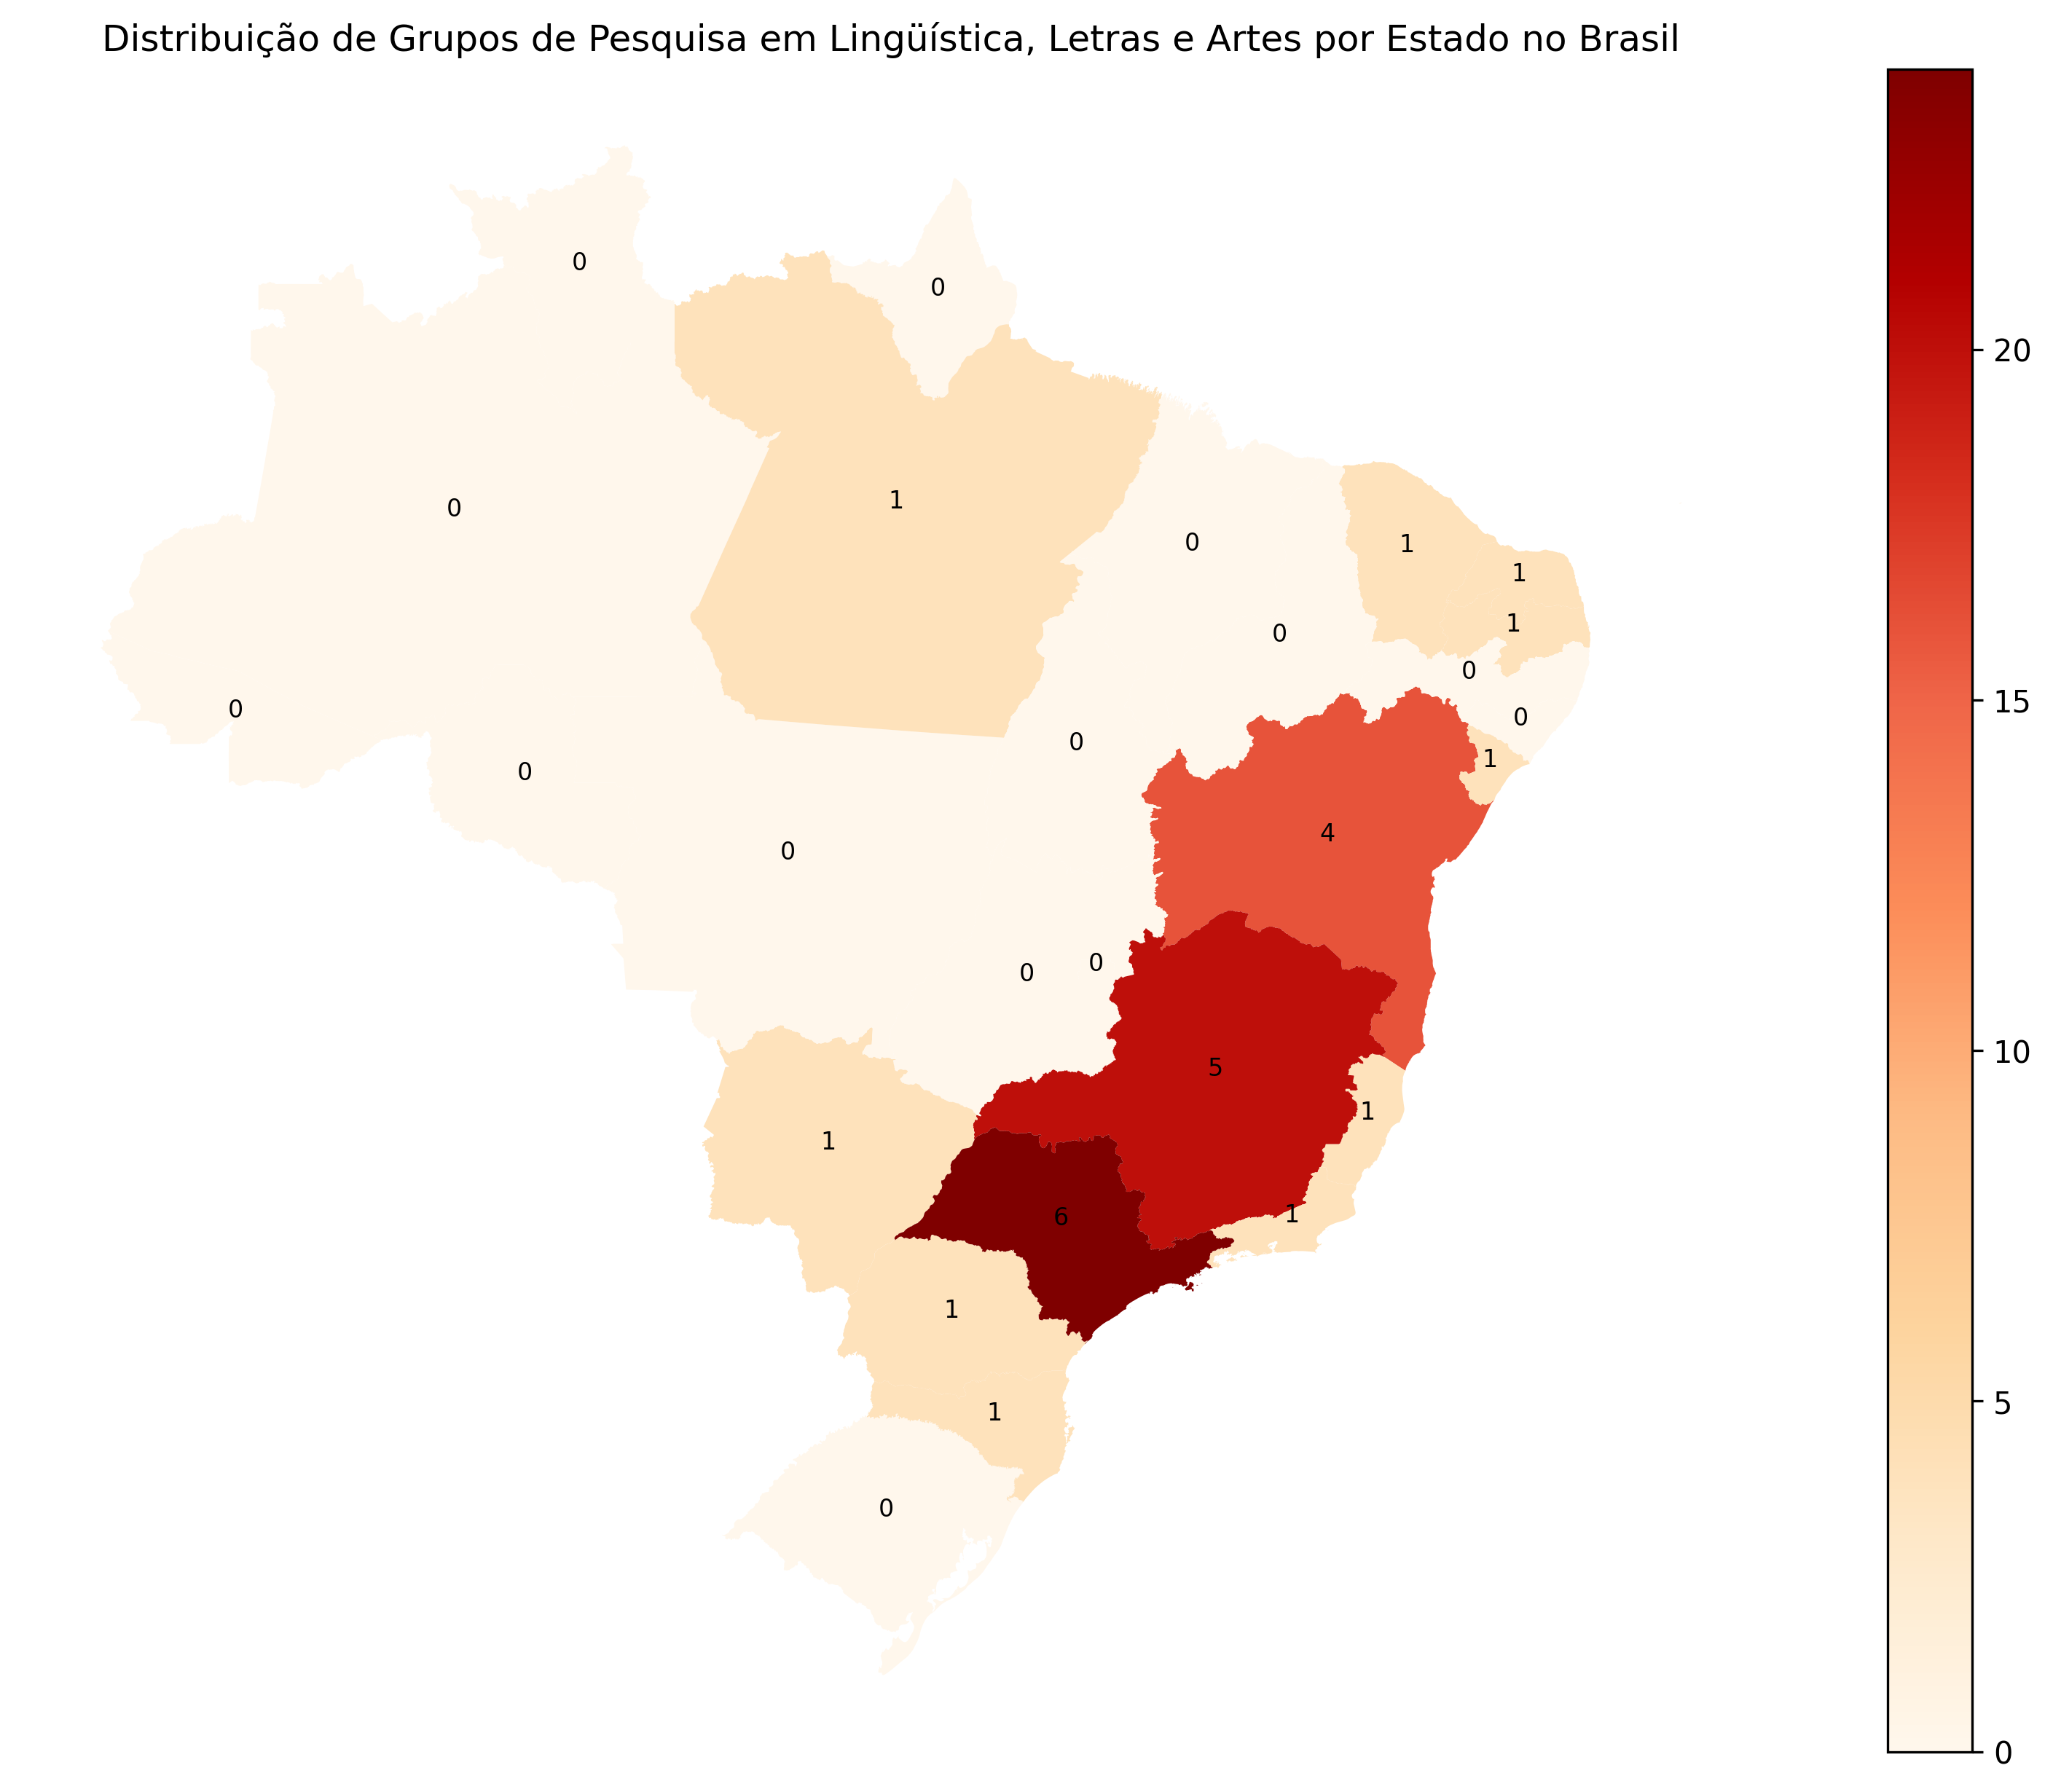
\includegraphics[keepaspectratio]{distribuicao_grupos_pesquisa_Lingüística,_Letras_e_Artes_brasil.png}}

\pandocbounded{\includegraphics[keepaspectratio]{distribuicao_grupos_pesquisa_Ciências_Sociais_Aplicadas_brasil.png}}

\subsubsection{Código}

\begin{Shaded}
\begin{Highlighting}[]
\CommentTok{\# Biblioteca}
\ImportTok{import}\NormalTok{ pandas }\ImportTok{as}\NormalTok{ pd}

\CommentTok{\# Banco de dados}
\NormalTok{matrix }\OperatorTok{=}\NormalTok{ pd.read\_csv(}\StringTok{\textquotesingle{}matrix\textquotesingle{}}\NormalTok{)}

\CommentTok{\# Geração de estatística descritiva por estado}
\NormalTok{frequencia\_por\_estado }\OperatorTok{=}\NormalTok{ matrix[}\StringTok{\textquotesingle{}UF\textquotesingle{}}\NormalTok{].value\_counts().reset\_index()}
\NormalTok{frequencia\_por\_estado.columns }\OperatorTok{=}\NormalTok{ [}\StringTok{\textquotesingle{}UF\textquotesingle{}}\NormalTok{, }\StringTok{\textquotesingle{}Frequencia Absoluta\textquotesingle{}}\NormalTok{]}
\NormalTok{frequencia\_por\_estado[}\StringTok{\textquotesingle{}Percentual\textquotesingle{}}\NormalTok{] }\OperatorTok{=}\NormalTok{ (frequencia\_por\_estado[}\StringTok{\textquotesingle{}Frequencia Absoluta\textquotesingle{}}\NormalTok{] }\OperatorTok{/}\NormalTok{ frequencia\_por\_estado[}\StringTok{\textquotesingle{}Frequencia Absoluta\textquotesingle{}}\NormalTok{].}\BuiltInTok{sum}\NormalTok{()) }\OperatorTok{*} \DecValTok{100}
\NormalTok{display(frequencia\_por\_estado)}

\CommentTok{\# Biblioteca de georreferenciamento}
\ImportTok{import}\NormalTok{ geopandas }\ImportTok{as}\NormalTok{ gpd}

\ControlFlowTok{try}\NormalTok{:}
    \CommentTok{\# Using a different known good source for Brazilian state boundaries}
\NormalTok{    brazil\_states }\OperatorTok{=}\NormalTok{ gpd.read\_file(}\StringTok{\textquotesingle{}https://raw.githubusercontent.com/codeforamerica/click\_that\_hood/master/public/data/brazil{-}states.geojson\textquotesingle{}}\NormalTok{)}
\NormalTok{    display(brazil\_states.head())}
\NormalTok{    brazil\_states.info()}
\ControlFlowTok{except} \PreprocessorTok{Exception} \ImportTok{as}\NormalTok{ e:}
    \BuiltInTok{print}\NormalTok{(}\SpecialStringTok{f"Could not load the GeoJSON file from the alternative source. Error: }\SpecialCharTok{\{}\NormalTok{e}\SpecialCharTok{\}}\SpecialStringTok{"}\NormalTok{)}
\NormalTok{    brazil\_states }\OperatorTok{=} \VariableTok{None} \CommentTok{\# Set to None if loading fails}
    
\NormalTok{brazil\_states\_merged }\OperatorTok{=}\NormalTok{ brazil\_states.merge(frequencia\_por\_estado, left\_on}\OperatorTok{=}\StringTok{\textquotesingle{}sigla\textquotesingle{}}\NormalTok{, right\_on}\OperatorTok{=}\StringTok{\textquotesingle{}UF\textquotesingle{}}\NormalTok{, how}\OperatorTok{=}\StringTok{\textquotesingle{}left\textquotesingle{}}\NormalTok{)}
\NormalTok{display(brazil\_states\_merged.head())}

\CommentTok{\# Plotagem}
\NormalTok{ax }\OperatorTok{=}\NormalTok{ brazil\_states\_merged.plot(column}\OperatorTok{=}\StringTok{\textquotesingle{}Percentual\textquotesingle{}}\NormalTok{, cmap}\OperatorTok{=}\StringTok{\textquotesingle{}OrRd\textquotesingle{}}\NormalTok{, legend}\OperatorTok{=}\VariableTok{True}\NormalTok{)}

\ControlFlowTok{for}\NormalTok{ index, row }\KeywordTok{in}\NormalTok{ brazil\_states\_merged.iterrows():}
\NormalTok{    centroid }\OperatorTok{=}\NormalTok{ row.geometry.centroid}
\NormalTok{    plt.text(centroid.x, centroid.y, }\BuiltInTok{str}\NormalTok{(}\BuiltInTok{int}\NormalTok{(row[}\StringTok{\textquotesingle{}Frequencia Absoluta\textquotesingle{}}\NormalTok{])), fontsize}\OperatorTok{=}\DecValTok{8}\NormalTok{, ha}\OperatorTok{=}\StringTok{\textquotesingle{}center\textquotesingle{}}\NormalTok{)}

\NormalTok{plt.title(}\StringTok{"Distribuição de Grupos de Pesquisa em IA por Estado no Brasil"}\NormalTok{)}
\NormalTok{ax.set\_axis\_off()}

\NormalTok{plt.savefig(}\StringTok{"distribuicao\_grupos\_pesquisa\_IA\_brasil.png"}\NormalTok{, dpi}\OperatorTok{=}\DecValTok{300}\NormalTok{, bbox\_inches}\OperatorTok{=}\StringTok{\textquotesingle{}tight\textquotesingle{}}\NormalTok{)}

\NormalTok{plt.show()}
\end{Highlighting}
\end{Shaded}

\subsection{Redes}\label{redes}

\subsubsection{Plotagem}\label{plotagem-1}

\pandocbounded{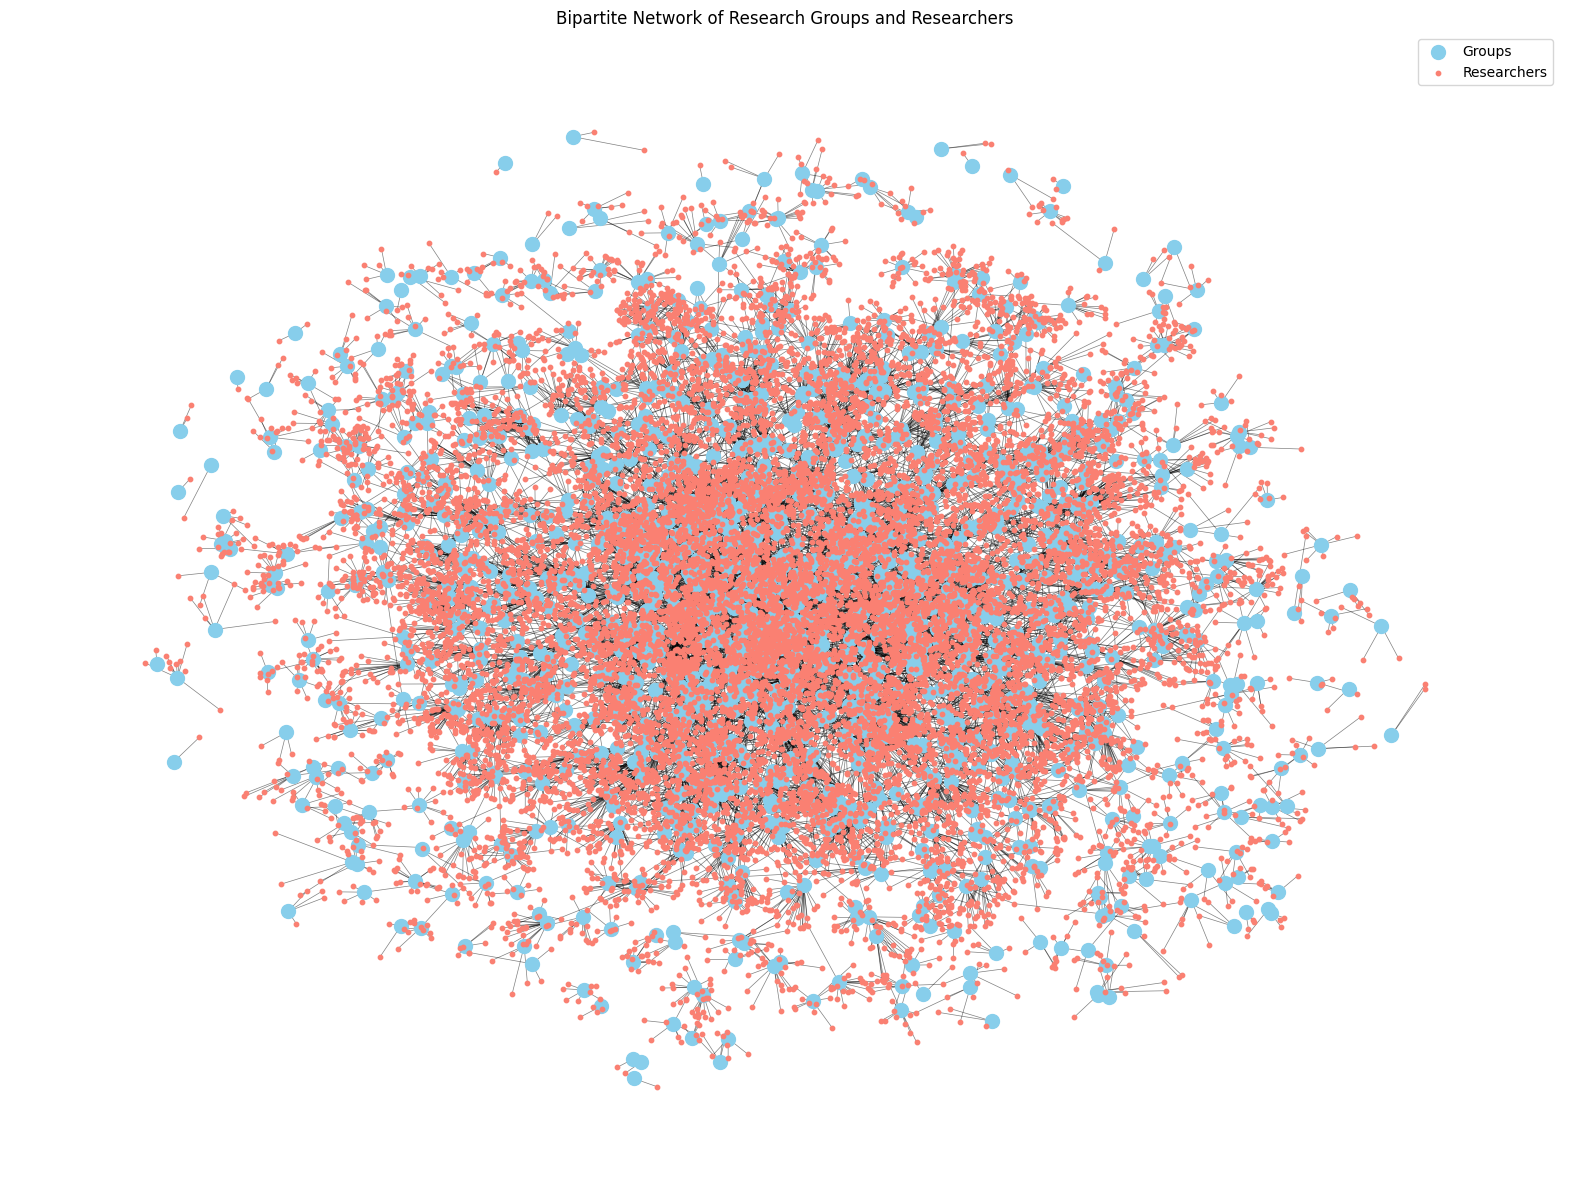
\includegraphics[keepaspectratio]{redes.png}}

\subsubsection{Código}\label{cuxf3digo-4}

\begin{Shaded}
\begin{Highlighting}[]
\ImportTok{import}\NormalTok{ pandas }\ImportTok{as}\NormalTok{ pd}
\ImportTok{import}\NormalTok{ networkx }\ImportTok{as}\NormalTok{ nx}
\ImportTok{import}\NormalTok{ matplotlib.pyplot }\ImportTok{as}\NormalTok{ plt}

\CommentTok{\# Carregar os dados}
\NormalTok{df\_relacional }\OperatorTok{=}\NormalTok{ pd.read\_csv(}\StringTok{\textquotesingle{}matrix\_relacionais\textquotesingle{}}\NormalTok{)}

\CommentTok{\# Pré{-}processar os dados}
\NormalTok{df\_filtered }\OperatorTok{=}\NormalTok{ df\_relacional[df\_relacional[}\StringTok{\textquotesingle{}Pesquisadores\textquotesingle{}}\NormalTok{] }\OperatorTok{!=} \StringTok{"Nenhum registro adicionado"}\NormalTok{]}

\CommentTok{\# Criar a rede bipartida}
\NormalTok{G }\OperatorTok{=}\NormalTok{ nx.Graph()}

\CommentTok{\# Add nodes for groups (bipartite=0)}
\NormalTok{group\_nodes }\OperatorTok{=}\NormalTok{ df\_filtered[}\StringTok{\textquotesingle{}ID\textquotesingle{}}\NormalTok{].unique()}
\NormalTok{G.add\_nodes\_from(group\_nodes, bipartite}\OperatorTok{=}\DecValTok{0}\NormalTok{)}

\CommentTok{\# Add nodes for researchers (bipartite=1)}
\NormalTok{researcher\_nodes }\OperatorTok{=}\NormalTok{ df\_filtered[}\StringTok{\textquotesingle{}Pesquisadores\textquotesingle{}}\NormalTok{].unique()}
\NormalTok{G.add\_nodes\_from(researcher\_nodes, bipartite}\OperatorTok{=}\DecValTok{1}\NormalTok{)}

\CommentTok{\# Add edges between groups and researchers}
\ControlFlowTok{for}\NormalTok{ index, row }\KeywordTok{in}\NormalTok{ df\_filtered.iterrows():}
\NormalTok{    group\_id }\OperatorTok{=}\NormalTok{ row[}\StringTok{\textquotesingle{}ID\textquotesingle{}}\NormalTok{]}
\NormalTok{    researcher\_name }\OperatorTok{=}\NormalTok{ row[}\StringTok{\textquotesingle{}Pesquisadores\textquotesingle{}}\NormalTok{]}
\NormalTok{    G.add\_edge(group\_id, researcher\_name)}

\CommentTok{\# Visualizar a rede}
\NormalTok{plt.rcParams[}\StringTok{\textquotesingle{}figure.figsize\textquotesingle{}}\NormalTok{] }\OperatorTok{=}\NormalTok{ (}\DecValTok{20}\NormalTok{, }\DecValTok{15}\NormalTok{) }\CommentTok{\# Increase figure size}

\CommentTok{\# Separate nodes by their bipartite attribute}
\NormalTok{groups }\OperatorTok{=}\NormalTok{ \{n }\ControlFlowTok{for}\NormalTok{ n, d }\KeywordTok{in}\NormalTok{ G.nodes(data}\OperatorTok{=}\VariableTok{True}\NormalTok{) }\ControlFlowTok{if}\NormalTok{ d[}\StringTok{"bipartite"}\NormalTok{] }\OperatorTok{==} \DecValTok{0}\NormalTok{\}}
\NormalTok{researchers }\OperatorTok{=} \BuiltInTok{set}\NormalTok{(G) }\OperatorTok{{-}}\NormalTok{ groups}

\CommentTok{\# Use a layout suitable for bipartite graphs}
\NormalTok{pos }\OperatorTok{=}\NormalTok{ nx.spring\_layout(G, k}\OperatorTok{=}\FloatTok{0.5}\NormalTok{, iterations}\OperatorTok{=}\DecValTok{50}\NormalTok{)}

\NormalTok{plt.figure(figsize}\OperatorTok{=}\NormalTok{(}\DecValTok{20}\NormalTok{, }\DecValTok{15}\NormalTok{))}

\CommentTok{\# Draw the nodes with different colors and sizes}
\NormalTok{nx.draw\_networkx\_nodes(G, pos, nodelist}\OperatorTok{=}\BuiltInTok{list}\NormalTok{(groups), node\_color}\OperatorTok{=}\StringTok{"skyblue"}\NormalTok{, node\_size}\OperatorTok{=}\DecValTok{100}\NormalTok{, label}\OperatorTok{=}\StringTok{"Groups"}\NormalTok{)}
\NormalTok{nx.draw\_networkx\_nodes(G, pos, nodelist}\OperatorTok{=}\BuiltInTok{list}\NormalTok{(researchers), node\_color}\OperatorTok{=}\StringTok{"salmon"}\NormalTok{, node\_size}\OperatorTok{=}\DecValTok{10}\NormalTok{, label}\OperatorTok{=}\StringTok{"Researchers"}\NormalTok{)}

\CommentTok{\# Draw the edges}
\NormalTok{nx.draw\_networkx\_edges(G, pos, width}\OperatorTok{=}\FloatTok{0.5}\NormalTok{, alpha}\OperatorTok{=}\FloatTok{0.5}\NormalTok{)}

\NormalTok{plt.title(}\StringTok{"Bipartite Network of Research Groups and Researchers"}\NormalTok{)}
\NormalTok{plt.axis(}\StringTok{"off"}\NormalTok{)}
\NormalTok{plt.legend()}
\NormalTok{plt.show()}
\end{Highlighting}
\end{Shaded}

\subsection{IA por área disciplinar}\label{ia-por-uxe1rea-disciplinar}

\pandocbounded{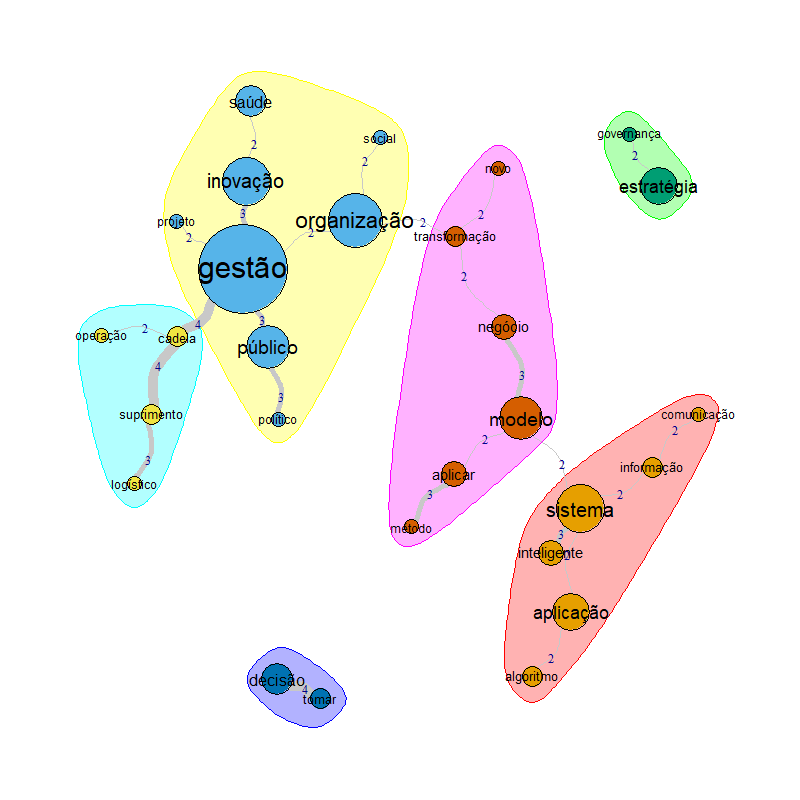
\includegraphics[keepaspectratio]{graph_simi_28.png}}

\pandocbounded{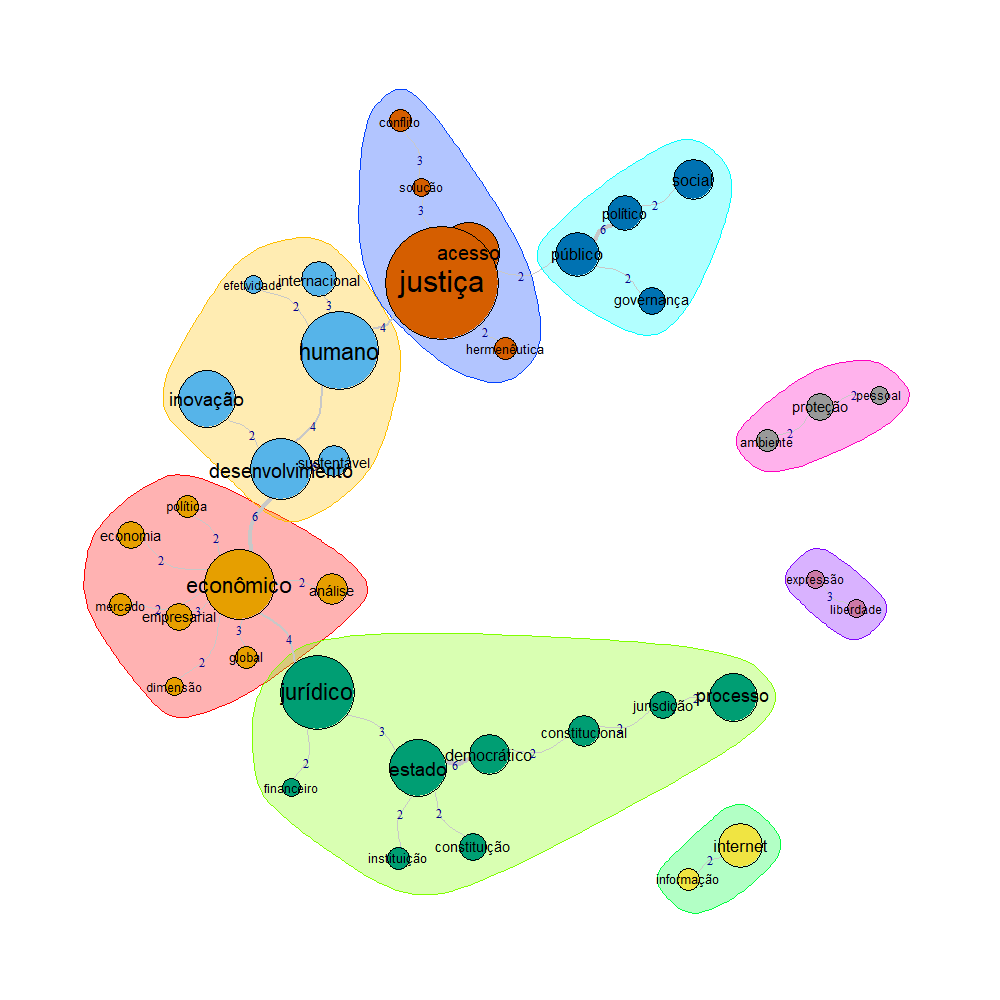
\includegraphics[keepaspectratio]{graph_simi_24.png}}

\subsection{IA por área disciplinar}\label{ia-por-uxe1rea-disciplinar-1}

\begin{itemize}
\tightlist
\item
  \textbf{Ciências Humanas}
\item
  \textbf{Ciências Sociais Aplicadas}
\item
  \textbf{Linguística, Letras e Artes}
\end{itemize}

\subsection{IA pelos seus usos}\label{ia-pelos-seus-usos}

\begin{itemize}
\tightlist
\item
  \textbf{IA como objeto}
\item
  \textbf{IA como técnica}
\item
  \textbf{Tecnologias digitais}
\end{itemize}

\section{Etapa 5. Formas de publicizar os
achados}\label{etapa-5.-formas-de-publicizar-os-achados}

\subsection{Relatórios e divulgação
científica}\label{relatuxf3rios-e-divulgauxe7uxe3o-cientuxedfica}

Em geral, a pesquisa se encerra com a escrita do relatório, que nos
permite desdobrar os achados em artigos, monografias, livros e outras
formas de publicizar os resultados.

Além de apresentações em seminários, uma dessas outras formas foi o
\href{https://scaimap.org/}{SCAI MAP}, em parceria com a rede coordenada
pela Prof.~Veridiana D. Cordeiro,
\href{https://understandingai.iea.usp.br/}{Understanding Artificial
Intelligence}.

\section{Muito obrigado!}\label{muito-obrigado}

Nossos e-mails:

\begin{itemize}
\tightlist
\item
  carolinabueno@usp.br
\item
  guilherme.olimpio@usp.br
\item
  gmc2406@usp.br
\end{itemize}

\subsection{Referências}\label{referuxeancias}

\phantomsection\label{refs.bib}

\phantomsection\label{refs}
\begin{CSLReferences}{1}{0}
\bibitem[\citeproctext]{ref-airoldi2021}
Airoldi, Massimo. 2021. \emph{Machine Habitus: Toward a Sociology of
Algorithms}. Polity.

\bibitem[\citeproctext]{ref-boden1996}
Boden, Margaret A. 1996. \emph{Artificial Intelligence}. Elsevier.

\bibitem[\citeproctext]{ref-cordeiro2023}
Cordeiro, Veridiana Domingos, Letícia Pereira Simões Gomes, e Leopoldo
Garcia Pinto Waizbort. 2023. {``A formação da sociologia digital:
emergência de uma nova especialidade na sociologia ou um campo para
repensar a própria sociologia?''} \emph{Plural} 30 (1): 5--22.
\url{https://doi.org/10.11606/issn.2176-8099.pcso.2023.211387}.

\bibitem[\citeproctext]{ref-costa2021}
Costa, Anna Helena, Leliane Nunes de Barros, Solange Oliveira Rezende,
Jaime S. Sichman, e Hugo Neri Munhoz. 2021. {``Trajetória acadêmica da
inteligência artificial no Brasil''}. Em \emph{Inteligência artificial :
avanços e tendências}. Instituto Estudos Avançados.

\bibitem[\citeproctext]{ref-esposito2022}
Esposito, Elena. 2022. \emph{Artificial communication: How algorithms
produce social intelligence}. MIT Press.

\bibitem[\citeproctext]{ref-lemieux2015}
Lemieux, Cyril. 2015. {``Problematizar''}. Em \emph{A pesquisa
sociológica}. Petrópolis: Vozes.

\bibitem[\citeproctext]{ref-liu2021}
Liu, Zheng. 2021. {``Sociological perspectives on artificial
intelligence: A typological reading''}. \emph{Sociology Compass} 15 (3):
e12851.

\bibitem[\citeproctext]{ref-omena2024}
Omena, Janna Joceli, Thais Lobo, Giulia Tucci, Elias Bitencourt, Emillie
de Keulenaar, Francisco W. Kerche, Jason Chao, Marius Liedtke, Mengying
Li, e Maria Luiza. 2024. {``Quali-quanti visual methods and political
bots''}. \emph{J. Digit. Social Res} 6 (1): 50--73.

\bibitem[\citeproctext]{ref-pasquinelli2023}
Pasquinelli, Matteo. 2023. \emph{The Eye of the Master: A Social History
of AI}. Verso.

\end{CSLReferences}




\end{document}
